\documentclass[twoside,twocolumn,10pt]{article}
\usepackage{fancyhdr}
\usepackage{geometry}
\usepackage{multicol}
\usepackage{abstract}
\usepackage{graphicx}
\graphicspath{{imagenes/}}
\usepackage{caption}
\usepackage{subcaption}
\usepackage{threeparttable}
\usepackage{titlesec}
\usepackage{ragged2e}
\usepackage{amssymb}
\usepackage{parskip}
\usepackage{amsmath}
\usepackage{newtxtext}
\usepackage{booktabs}
\usepackage{array}
\usepackage[spanish,es-tabla]{babel}
\usepackage[
	backend=biber,
	style=chem-acs,
	articletitle=false,
	maxnames=4,
	minnames=1
]{biblatex}
\usepackage[version=4]{mhchem}
\usepackage{xurl}
\usepackage{placeins} 
\addbibresource{references.bib}
\raggedbottom
\setcounter{page}{1}

\renewcommand{\topfraction}{0.85}
\renewcommand{\dbltopfraction}{0.85}
\renewcommand{\textfraction}{0.1}
\renewcommand{\floatpagefraction}{0.75}
\renewcommand{\dblfloatpagefraction}{0.75}
\setlength{\textfloatsep}{12pt plus 2pt minus 2pt}
\setlength{\dbltextfloatsep}{12pt plus 2pt minus 2pt}

\newcolumntype{L}[1]{>{\raggedright\arraybackslash}p{#1}}
\newcolumntype{C}[1]{>{\centering\arraybackslash}p{#1}}
\newcolumntype{R}[1]{>{\raggedleft\arraybackslash}p{#1}}

\usepackage[font=footnotesize, labelfont=bf, justification=raggedright, format=plain]{caption}
\captionsetup[table]{labelsep=colon, justification=justified}
\captionsetup[figure]{labelsep=colon, justification=justified, name=Fig.}

\geometry{letterpaper, left=0.8in, right=0.8in, top=1in, bottom=1in}
\setlength{\columnsep}{20pt}

\renewcommand{\abstractname}{\hspace{1.3em}\textbf{Resumen}}
\titleformat{\section}{\large\bfseries\uppercase}{\thesection.}{1em}{}
\titleformat{\subsection}{\normalfont\bfseries\itshape\flushleft}{\thesubsection}{0.8em}{}
\titleformat{\subsubsection}{\normalfont\bfseries\itshape\flushleft}{\thesubsubsection}{1em}{}
\renewcommand{\abstractnamefont}{\normalfont\fontsize{14}{20}\bfseries}
\renewcommand{\absnamepos}{flushleft}
\renewcommand{\abstracttextfont}{\normalfont\fontsize{11}{13}\selectfont}

\hyphenpenalty=10000
\exhyphenpenalty=10000
\sloppy

\pagestyle{fancy}
\fancyhf{}
\fancyhead[C]{\small Hidrocarburos: reacciones y obtenciones}
\fancyhead[CE]{\small Proyecto de Química Orgánica  (2026)}
\fancyfoot[C]{\thepage}

\fancypagestyle{firstpage}{
  \fancyhf{}
  \fancyhead[LO]{\small Ingeniería Ambiental, FAMARENA-UD}
  \fancyhead[RO]{\small 2026-III}


  \renewcommand{\headrulewidth}{0.4pt}
  \renewcommand{\footrulewidth}{0.4pt}
}

\title{\fontsize{16}{20}\selectfont\textbf{Hidrocarburos: reacciones y obtenciones}}

\author{
    \fontsize{12}{14}\selectfont
    Vanessa Valentina Sánchez Ulloa\textsuperscript{}, Sharay Quiroga Acero\textsuperscript{}, Alejandra Valeria Ulloa Soteldo\textsuperscript{}, Zharith Garzón\textsuperscript{}\\[1ex]
    \fontsize{12}{14}\selectfont
    \textsuperscript{}Facultad de Medio Ambiente y Recursos Naturales,\\ Universidad Distrital Francisco José de Caldas, Bogotá, Colombia
}
\date{}

\begin{document}

\twocolumn[
\begin{@twocolumnfalse}
\vspace{-0.5cm}
\raggedright
{\fontsize{11}{13}\selectfont{Artículo de investigación}}
\vspace{-0.8cm}
\maketitle
\thispagestyle{firstpage}
\begin{abstract}
\fontsize{11}{13}\selectfont
\vspace{1em}
\justifying
Los hidrocarburos solo interactúan entre sí por fuerzas de London y sus enlaces C–H son poco reactivos; este trabajo examina cómo esas dos características se reflejan en datos reales. Se estudiaron cinco alcanos (pentano, isopentano, hexano, heptano y octano), tres alquenos (cis-pent-2-eno, 2-metilpent-2-eno y hex-1-eno) y dos cicloalquenos (ciclopropeno y ciclobuteno), con 100 reacciones en las que actúan como reactivo y 100 en las que se obtienen, tomadas de CAS SciFinder. En la serie lineal el punto de ebullición sube 29.8~\textdegree C por carbono y la ramificación lo reduce; en los productos, Peb $\approx$ 1.02·PM + 39 ($R^2$ = 0.68) y la presión de vapor cae con el punto de ebullición ($r$ = $-$0.86). Los alcanos reaccionan sobre todo mediante metales u otras especies que rompen el enlace C–H (organometálica 33\,\%, radicalaria 15\,\%), los alquenos por adición y el ciclopropeno por cicloadición, mientras que los hidrocarburos se obtienen principalmente por reducción (62\,\%) y eliminación (25\,\%). El medio neutro predomina (0.56) y el 62\,\% de las reacciones usa catalizador.

\vspace{-0.1cm}
\noindent\textbf{Palabras clave:}
 alcanos, alquenos, análisis de datos, activación C–H, Colab, fuerzas de London, SciFinder.
\end{abstract}
\vspace{1cm}
\end{@twocolumnfalse}
]

\section{Introducción}
\fontsize{12}{14}\selectfont
Los hidrocarburos son la base de los combustibles y la principal materia prima de la industria química. Al estar formados solo por carbono e hidrógeno, son moléculas casi apolares: no forman puentes de hidrógeno y sus propiedades físicas dependen del tamaño y de la forma de la molécula. Químicamente, los alcanos son poco reactivos porque sus enlaces C–H son fuertes y no polares, mientras que los alquenos tienen un doble enlace rico en electrones que reacciona con facilidad.
Este trabajo usa la información de CAS SciFinder \cite{Gabrielson2018,CAS2026} para entender mejor ¿cómo cambian sus propiedades con el número de carbonos, la ramificación y la insaturación?, ¿qué mecanismos siguen cuando reaccionan y cuáles cuando se obtienen? y ¿qué condiciones (medio, temperatura, catalizador y solvente) necesitan? estos hidrocarburos para asi entenderlos mejor.

\section{Revisión Literatura}
\fontsize{12}{14}\selectfont
\textbf{El problema del enlace C–H.} Labinger y Bercaw \cite{Labinger2002} explican que los alcanos son difíciles de transformar porque sus enlaces C–H son fuertes y poco polares, y muestran cómo los complejos de metales de transición pueden romperlos en condiciones suaves y con selectividad; por eso proponen que los alcanos podrían llegar a ser materia prima directa para la industria química.

\textbf{Funcionalización por radicales.} Otra vía es usar luz y un fotocatalizador. Holmberg-Douglas y Nicewicz \cite{HolmbergDouglas2022} revisan las reacciones de funcionalización C–H por fotocatálisis redox y señalan que los enlaces C–H alifáticos no activados, con energías de disociación mayores de 92~kcal/mol, siguen siendo los más difíciles de transformar.

\textbf{Hidrogenación.} La reducción de dobles y triples enlaces es la ruta más común para obtener alcanos. Gong \textit{et al.} \cite{Gong2025} revisan catalizadores heterogéneos de metales no preciosos para hidrogenación selectiva por vías térmica, fotocatalítica y electrocatalítica.

\textbf{Cicloalquenos tensionados.} El ciclopropeno tiene un anillo de tres carbonos muy tensionado que lo hace reaccionar con tetrazinas por cicloadición; Kumar \textit{et al.} \cite{Kumar2018} usaron grupos protectores voluminosos para bloquear esa reacción y activarla solo al retirarlos, lo que muestra lo reactivo que es este anillo.

\section{Metodología}
\fontsize{12}{14}\selectfont
\subsection{Datos}
Para cada hidrocarburo se registraron en CAS SciFinder sus propiedades (PM, Pf, Peb, $\rho$, pKa, $\mu$, solubilidad en agua y Pv), diez reacciones donde es reactivo y diez donde es producto, con sus reactivos, catalizadores, solventes, temperatura, tiempo, presión y medio. La información se organizó en Excel con tres hojas (Sustancias, Reacciones con 203 filas y Obtenciones con 122 filas, una fila por paso). Se organizaron de la siguiente manera: una tabla por hoja, sin celdas combinadas, unidades solo en el encabezado, NA para los datos inexistentes y sin mezclar texto y números en una columna. La temperatura ``ambiente'' se tomó como 25~\textdegree C, los rangos como su promedio y las rampas como su valor máximo.

\subsection{Clasificación por mecanismo}
Cada reacción se asignó a un tipo según su mecanismo principal: sustitución nucleofílica, electrofílica o radicalaria; adición nucleofílica, electrofílica o radicalaria; eliminación; condensación y redox. Los hidrocarburos requirieron dos categorías adicionales: \textit{cicloadición (pericíclica)}, para las reacciones de Diels–Alder y [2+2], y \textit{organometálica e isomerización}, para las transformaciones mediadas por metales de transición (activación C–H, acoplamientos de Heck, isomerizaciones catalíticas).

\subsection{Análisis}
El análisis se programó en Google Colab con pandas \cite{McKinney2010}, Matplotlib \cite{Hunter2007}, seaborn \cite{Waskom2021}, SciPy \cite{Virtanen2020} y Plotly. Se calcularon correlaciones de Pearson y Spearman, regresiones lineales, la prueba de Mann-Whitney y proporciones con intervalo de confianza de Wilson del 95\,\% \cite{Wilson1927,Brown2001}. Los tipos de gráfica se escogieron según el tipo de variable \cite{Datavizcatalogue} y se usó la paleta viridis, con un color fijo para cada variable \cite{Datawrapper}.

\section{Resultados y Discusión}
\fontsize{12}{14}\selectfont
\subsection{Estructura y propiedades físicas}

\begin{table*}[!t]
	\centering
	\caption{Propiedades de los diez hidrocarburos, ordenados por peso molecular (CAS SciFinder). NA: dato no disponible. Los valores marcados con $^\dagger$ deben verificarse.}
	\label{tab:sustancias}
	\begin{tabular}{llrrrrrr}
		\toprule
		\textbf{Hidrocarburo} & \textbf{Tipo} & \textbf{PM (g/mol)} & \textbf{Pf (\textdegree C)} & \textbf{Peb (\textdegree C)} & \textbf{$\rho$ (g/cm\textsuperscript{3})} & \textbf{Sol. (mol/L)} & \textbf{Pv (Pa)} \\
		\midrule
		Ciclopropeno & Cicloalqueno & 40.06 & NA & 35.5$^\dagger$ & 2.754$^\dagger$ & 5.7$\times$10$^{-2}$ & 5.9$\times$10$^{5}$ \\
		Ciclobuteno & Cicloalqueno & 54.09 & NA & 2.0 & 0.807 & 2.1$\times$10$^{-2}$ & 2.3$\times$10$^{5}$ \\
		cis-Pent-2-eno & Alqueno & 70.13 & $-$187.0 & 35.5 & 0.958$^\dagger$ & 1.5$\times$10$^{-3}$ & 6.5$\times$10$^{4}$ \\
		Pentano & Alcano & 72.15 & $-$129.7 & 36.1 & 0.626 & 5.7$\times$10$^{-4}$ & 2.6$\times$10$^{6\dagger}$ \\
		Isopentano & Alcano ramif. & 72.15 & $-$159.9 & 27.8 & 0.620 & 6.7$\times$10$^{-4}$ & 7.9$\times$10$^{4}$ \\
		2-Metilpent-2-eno & Alqueno ramif. & 84.16 & $-$135.0 & 67.3 & 0.689 & 4.1$\times$10$^{-4}$ & 2.1$\times$10$^{4}$ \\
		Hex-1-eno & Alqueno & 84.16 & $-$139.7 & 63.4 & 0.673 & 5.6$\times$10$^{-4}$ & 1.7$\times$10$^{5}$ \\
		Hexano & Alcano & 86.18 & $-$94.3 & 68.7 & 0.655 & 6.5$\times$10$^{-4}$ & 1.4$\times$10$^{5}$ \\
		Heptano & Alcano & 100.20 & $-$91.0 & 98.0 & 0.680 & 3.4$\times$10$^{-5}$ & 5.0$\times$10$^{5\dagger}$ \\
		Octano & Alcano & 114.23 & $-$56.8 & 125.7 & 0.699 & 6.0$\times$10$^{-6}$ & 1.5$\times$10$^{3}$ \\
		\bottomrule
	\end{tabular}
\end{table*}

La Tabla~\ref{tab:sustancias} muestra que, dentro de los alcanos lineales, el punto de ebullición y el de fusión aumentan con la longitud de la cadena, y que la solubilidad en agua es muy baja en todos los casos (entre 10$^{-6}$ y 10$^{-2}$~mol/L), como se espera de moléculas apolares.

\begin{figure*}[!t]
\centering
\begin{subfigure}[t]{0.5\textwidth}\centering
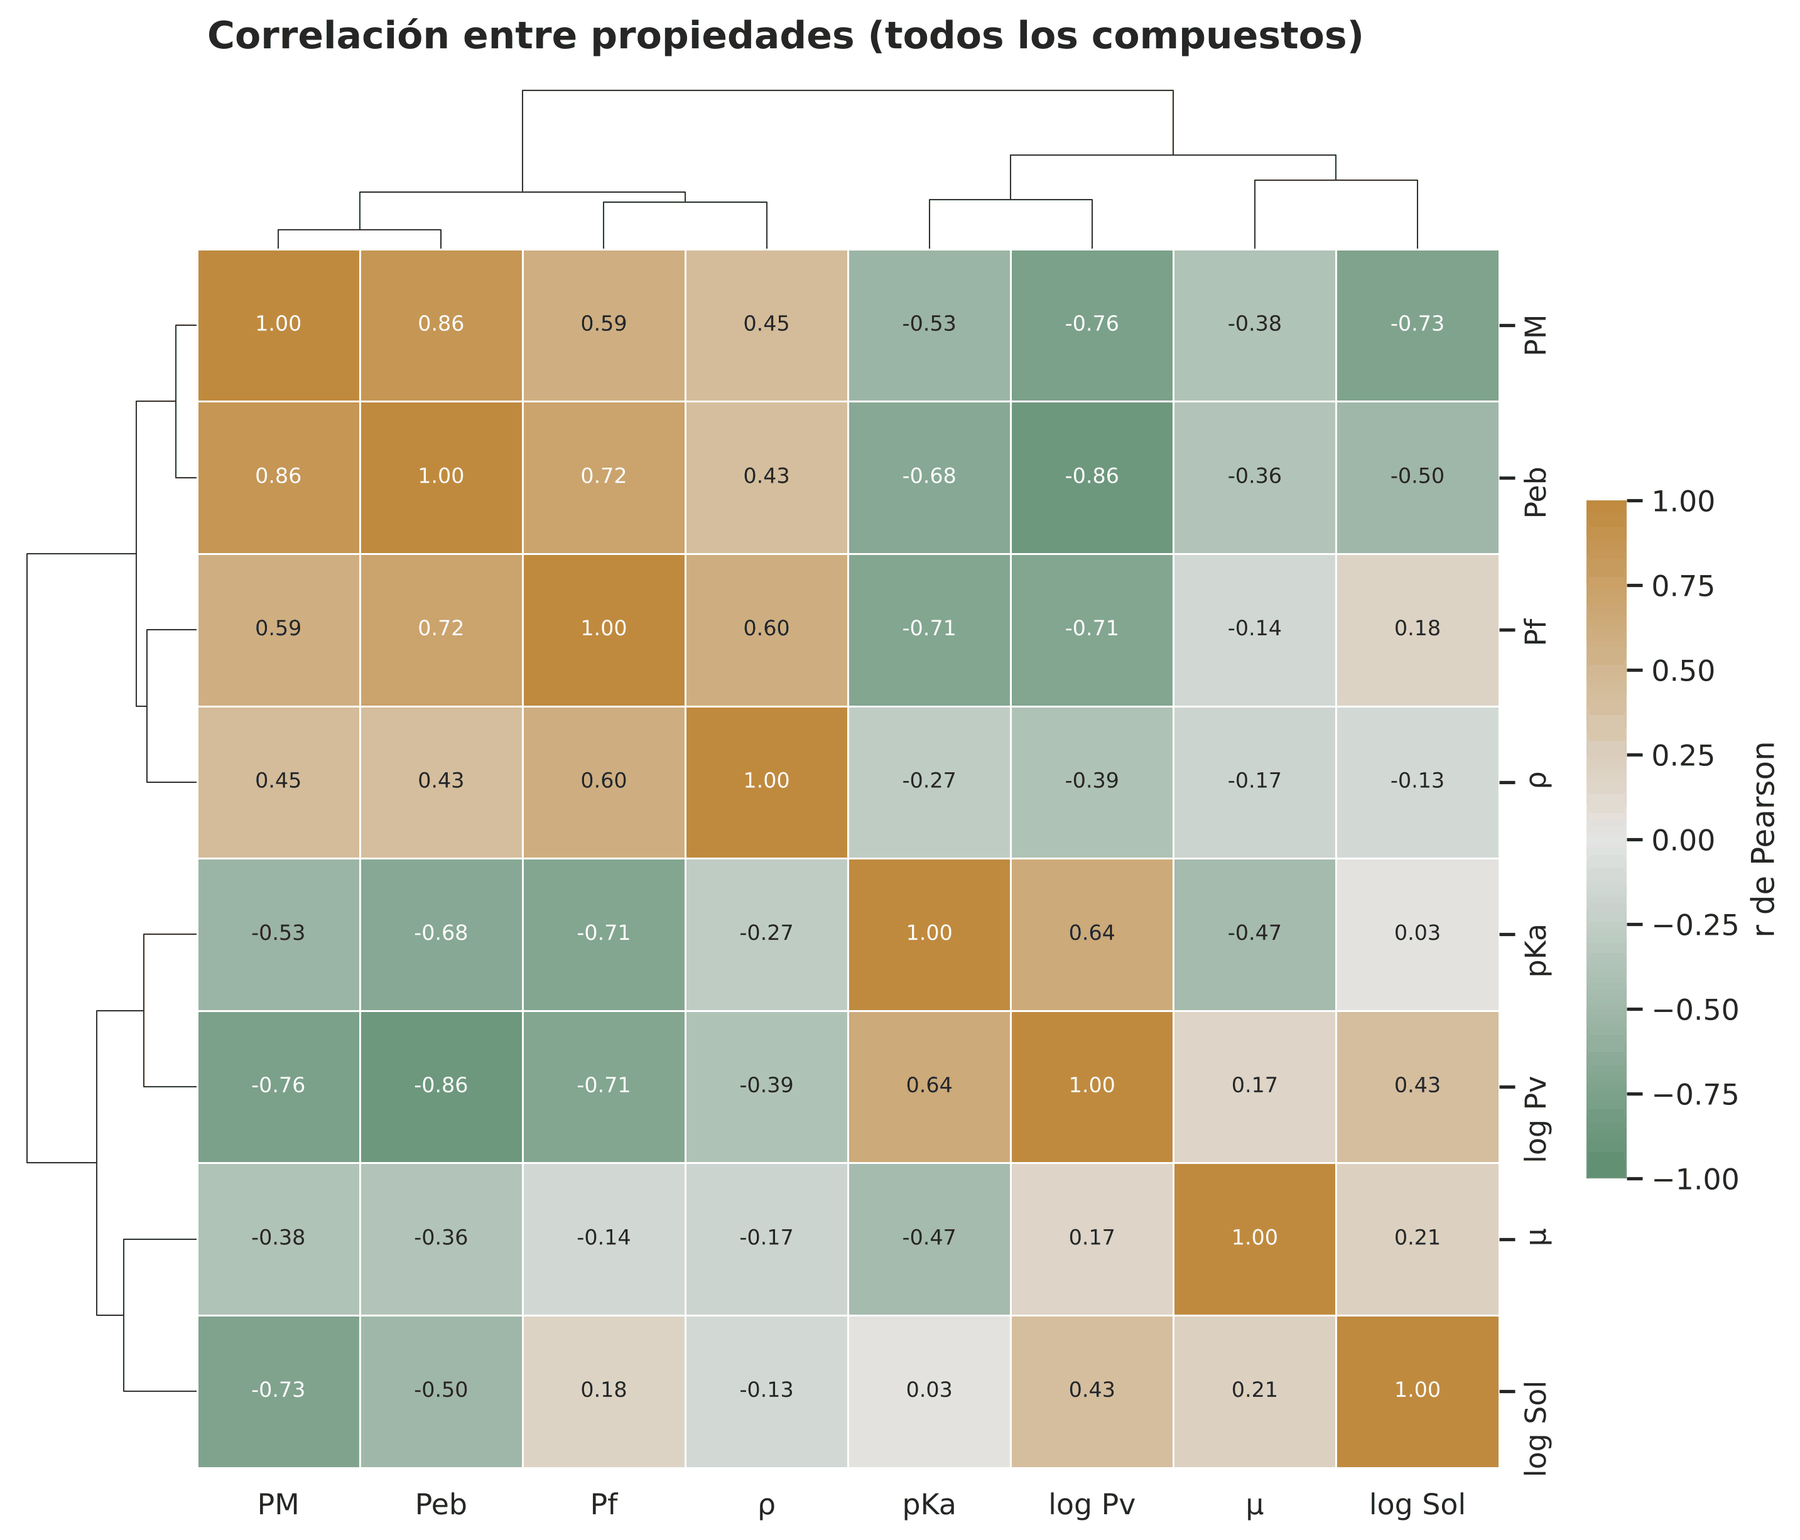
\includegraphics[width=\linewidth]{01_mapa_correlacion.png}
\caption{Correlación de Pearson con dendrograma (todos los compuestos).}
\label{fig:corr}
\end{subfigure}\hfill
\begin{subfigure}[t]{0.48\textwidth}\centering
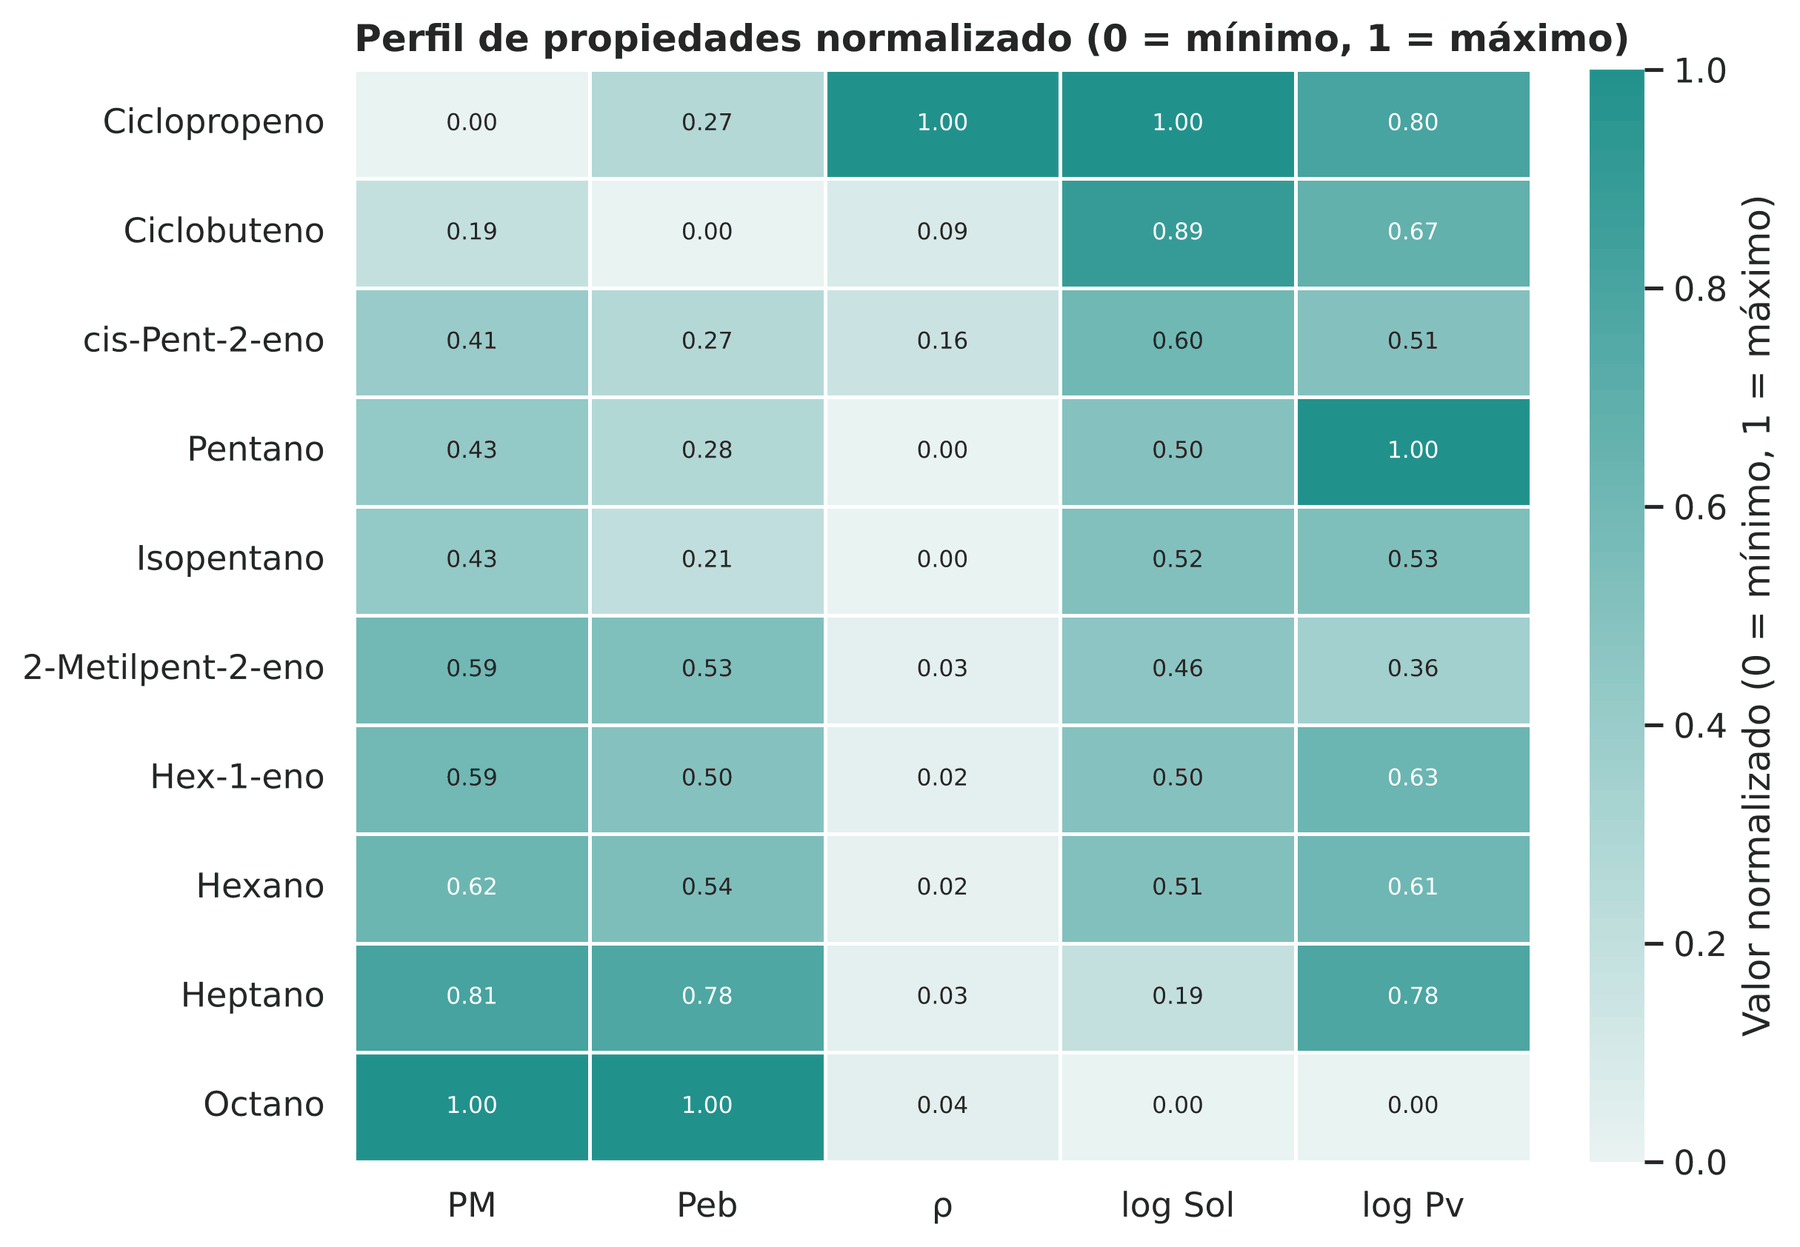
\includegraphics[width=\linewidth]{02_propiedades_normalizadas.png}
\caption{Propiedades normalizadas de los diez hidrocarburos.}
\label{fig:norm}
\end{subfigure}
\caption{Visión general de las propiedades. En (b), 0 corresponde al valor mínimo del grupo y 1 al máximo; Pf y $\mu$ se excluyen por datos faltantes.}
\label{fig:general}
\end{figure*}

La matriz de correlación (Fig.~\ref{fig:corr}) confirma que el tamaño gobierna la volatilidad: PM–Peb ($r$ = 0.86) y Peb–log Pv ($r$ = $-$0.86) son las parejas más fuertes, y el dendrograma separa un grupo de propiedades de tamaño (PM, Peb, Pf, $\rho$) de otro de volatilidad. En el perfil normalizado (Fig.~\ref{fig:norm}) el octano ocupa el extremo de mayor PM y Peb y menor solubilidad y presión de vapor.

\begin{figure*}[!t]
\centering
\begin{subfigure}[t]{0.52\textwidth}\centering
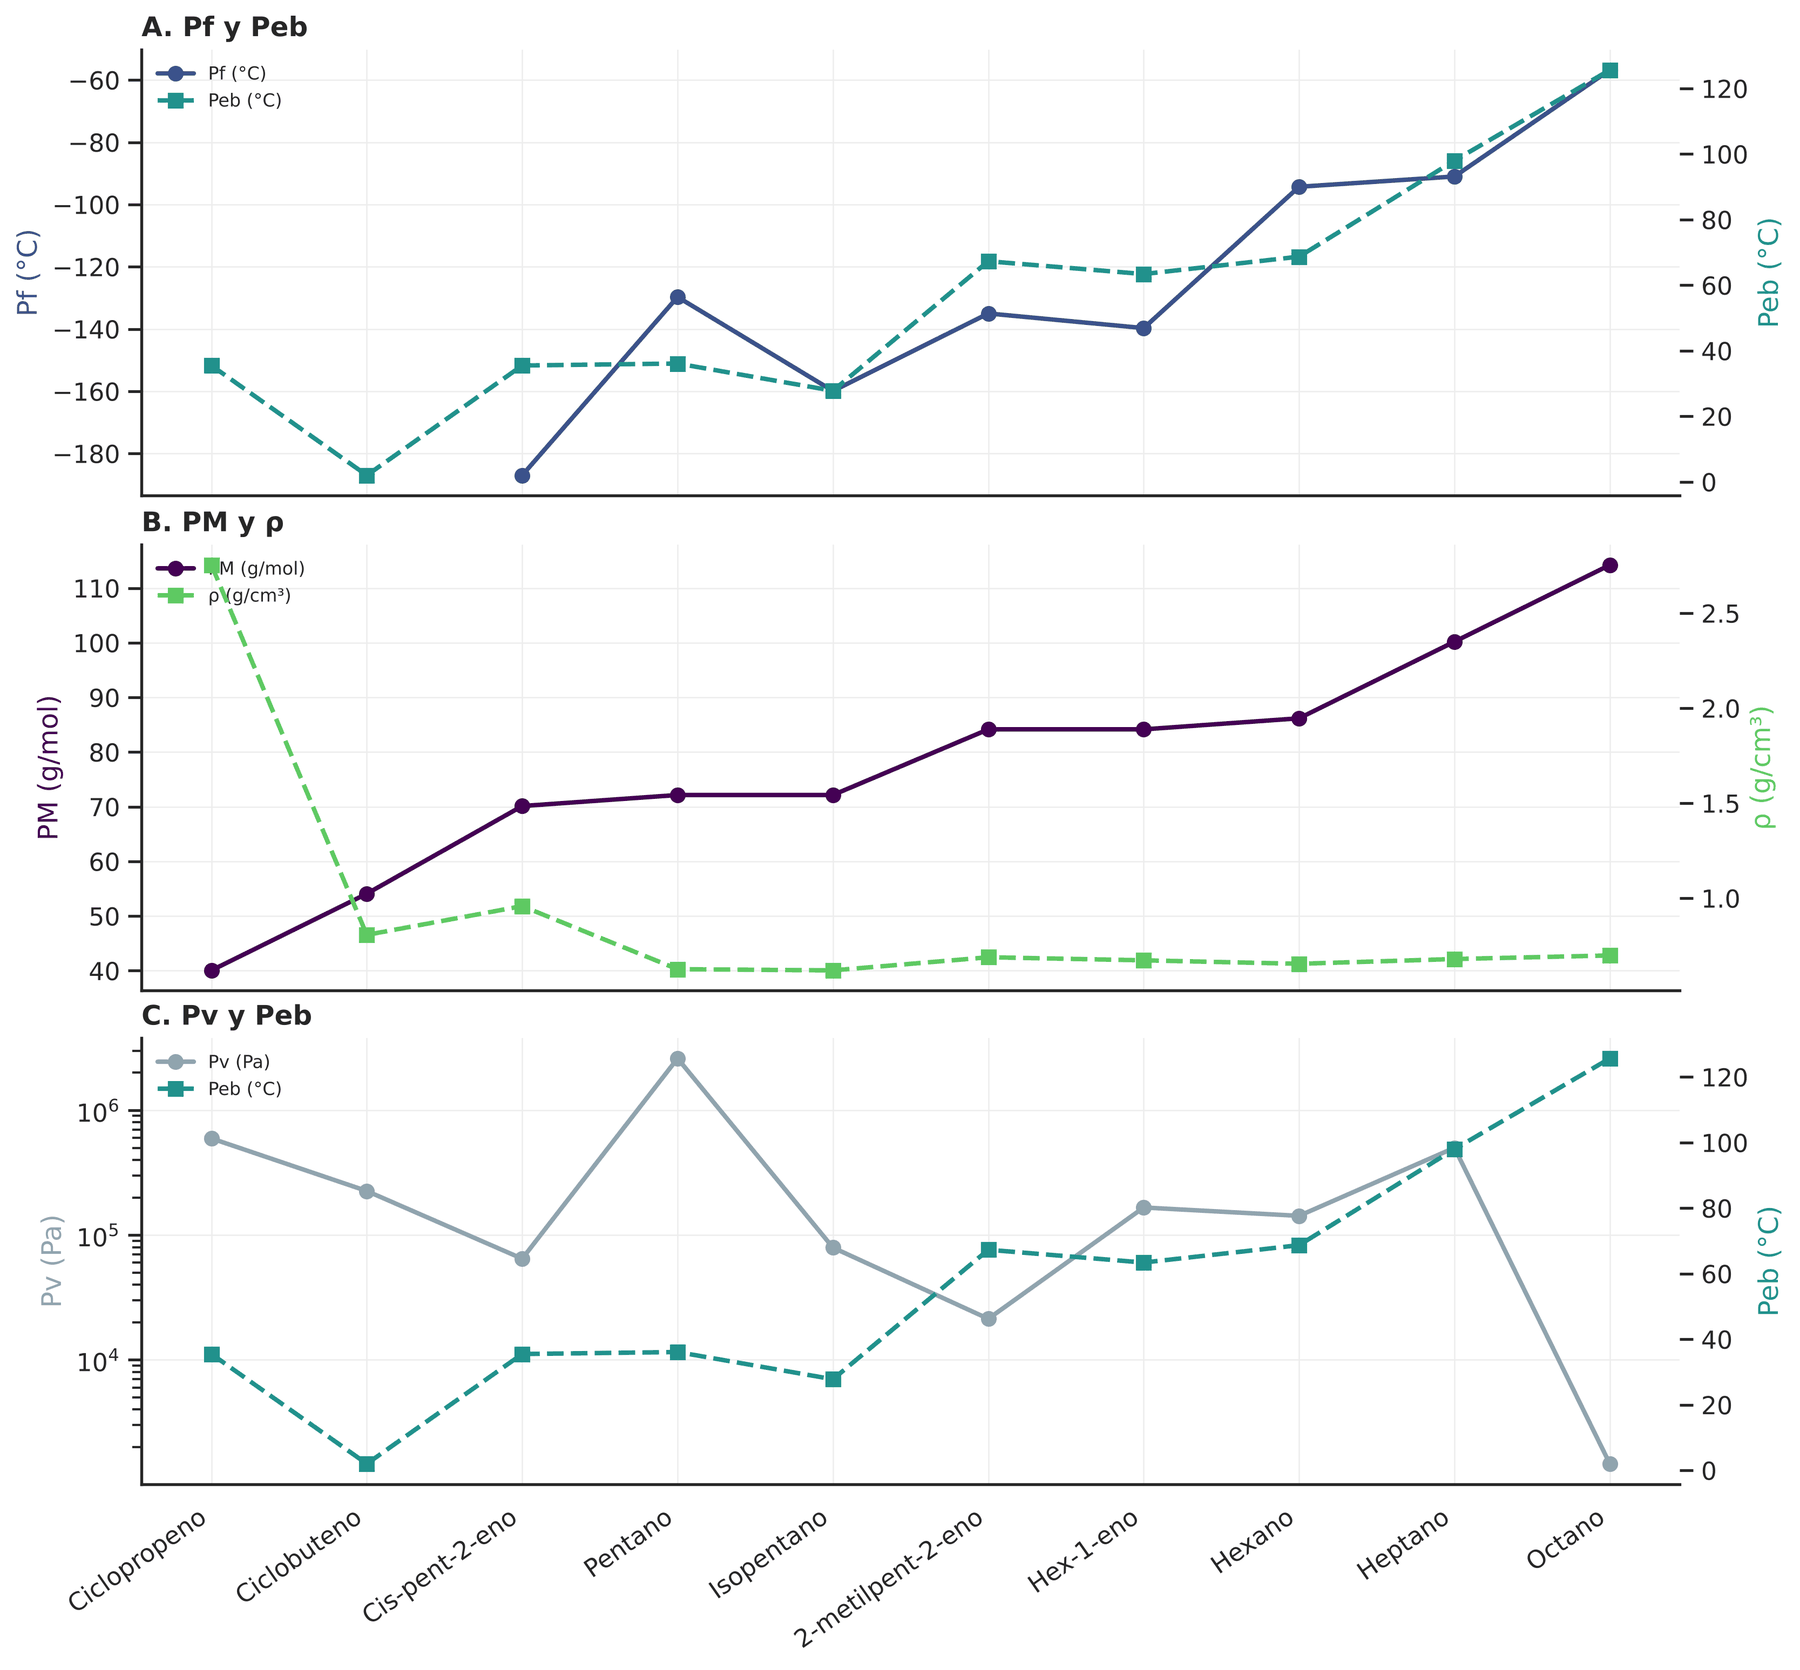
\includegraphics[width=\linewidth]{03_doble_eje_propiedades.png}
\caption{Pares de propiedades con doble eje: Pf y Peb (A), PM y $\rho$ (B), Pv y Peb (C).}
\label{fig:doble}
\end{subfigure}\hfill
\begin{subfigure}[t]{0.46\textwidth}\centering
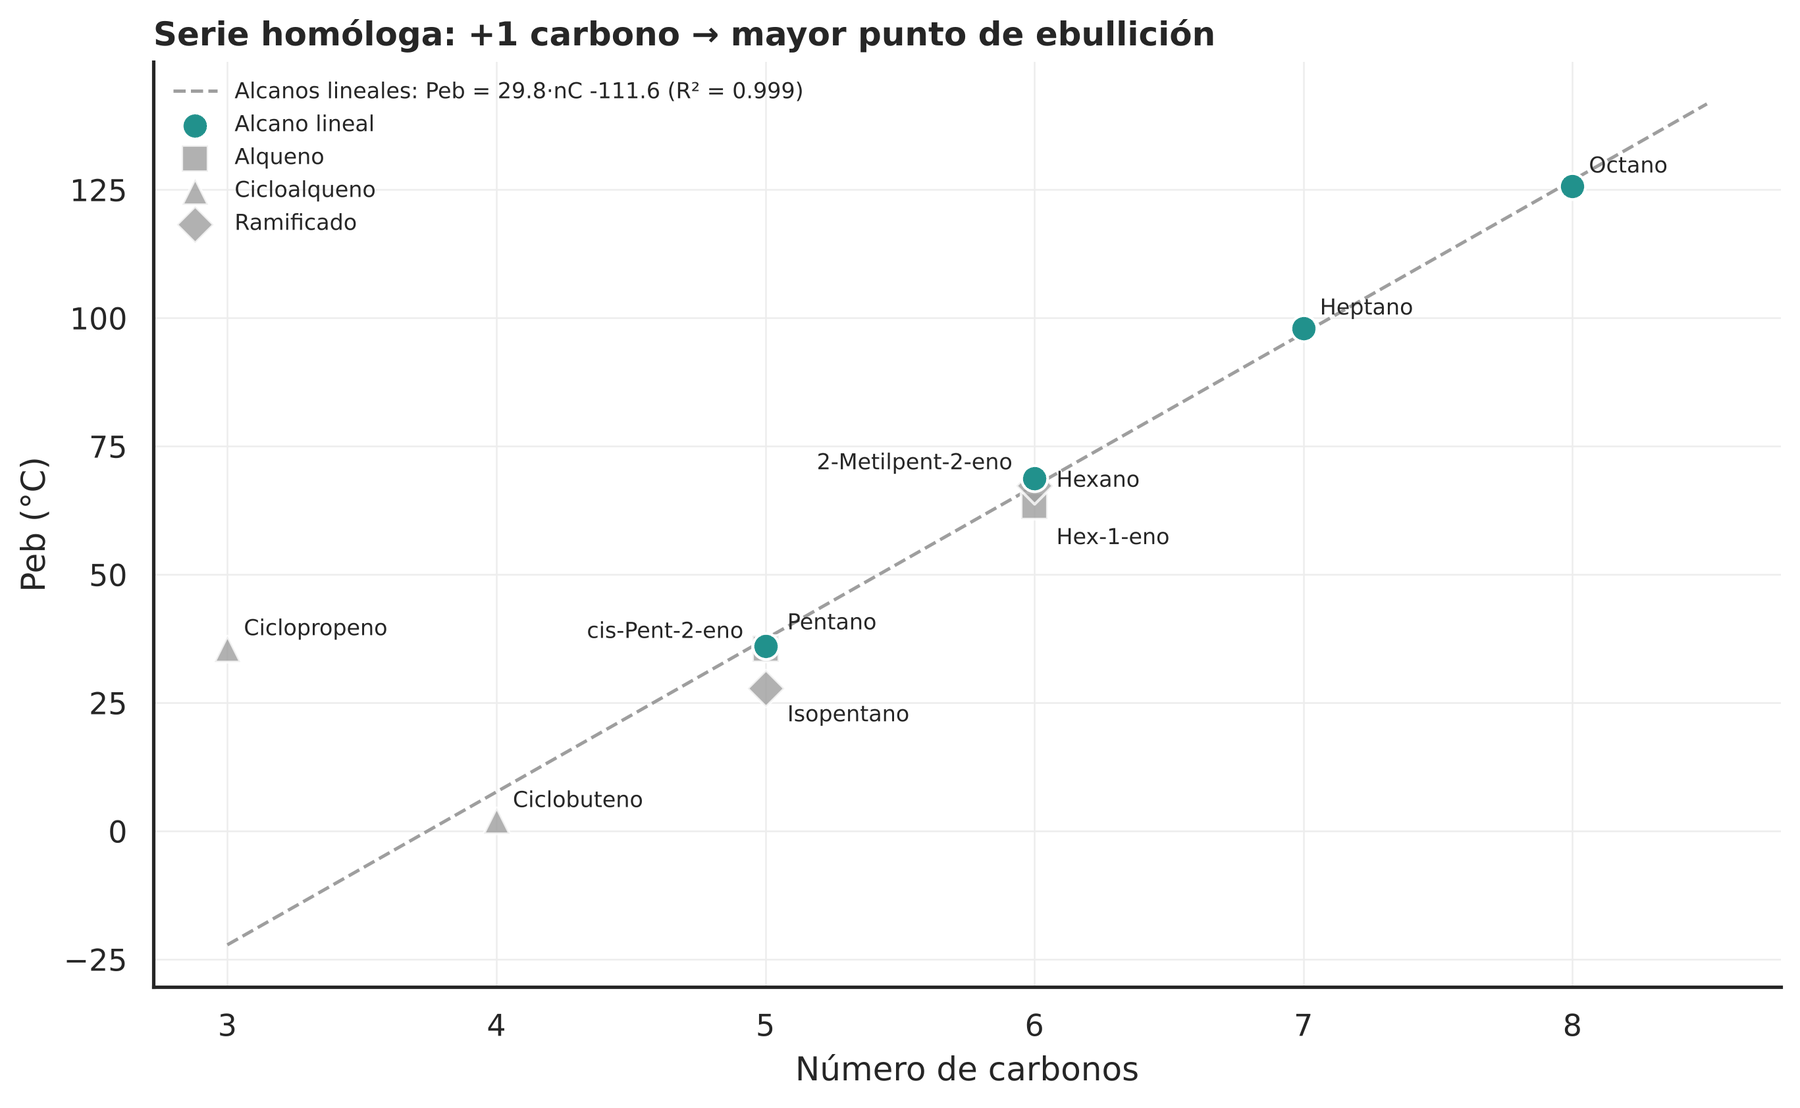
\includegraphics[width=\linewidth]{04_tendencia_homologa.png}
\caption{Peb frente al número de carbonos.}
\label{fig:homologa}
\end{subfigure}
\caption{Efecto de la estructura. Los hidrocarburos se ordenan por peso molecular en (a); en (b) la recta se ajusta solo a los alcanos lineales.}
\label{fig:estructura}
\end{figure*}

El Pf y el Peb crecen juntos con el tamaño (Spearman $\rho_s$ = 0.90, $p$ = 0.002; Fig.~\ref{fig:doble}). En la serie de alcanos lineales cada carbono añadido sube el Peb en 29.8~\textdegree C ($R^2$ = 0.999, $n$ = 4; Fig.~\ref{fig:homologa}), por el aumento de la superficie de contacto y de las fuerzas de London. La forma de la molécula también cuenta el isopentano, ramificado, hierve 8.3~\textdegree C por debajo del pentano, y el hex-1-eno 5.3~\textdegree C por debajo del hexano.

\subsection{Volatilidad y tamaño de los productos}

\begin{figure*}[!t]
\centering
\begin{subfigure}[t]{0.329\textwidth}\centering
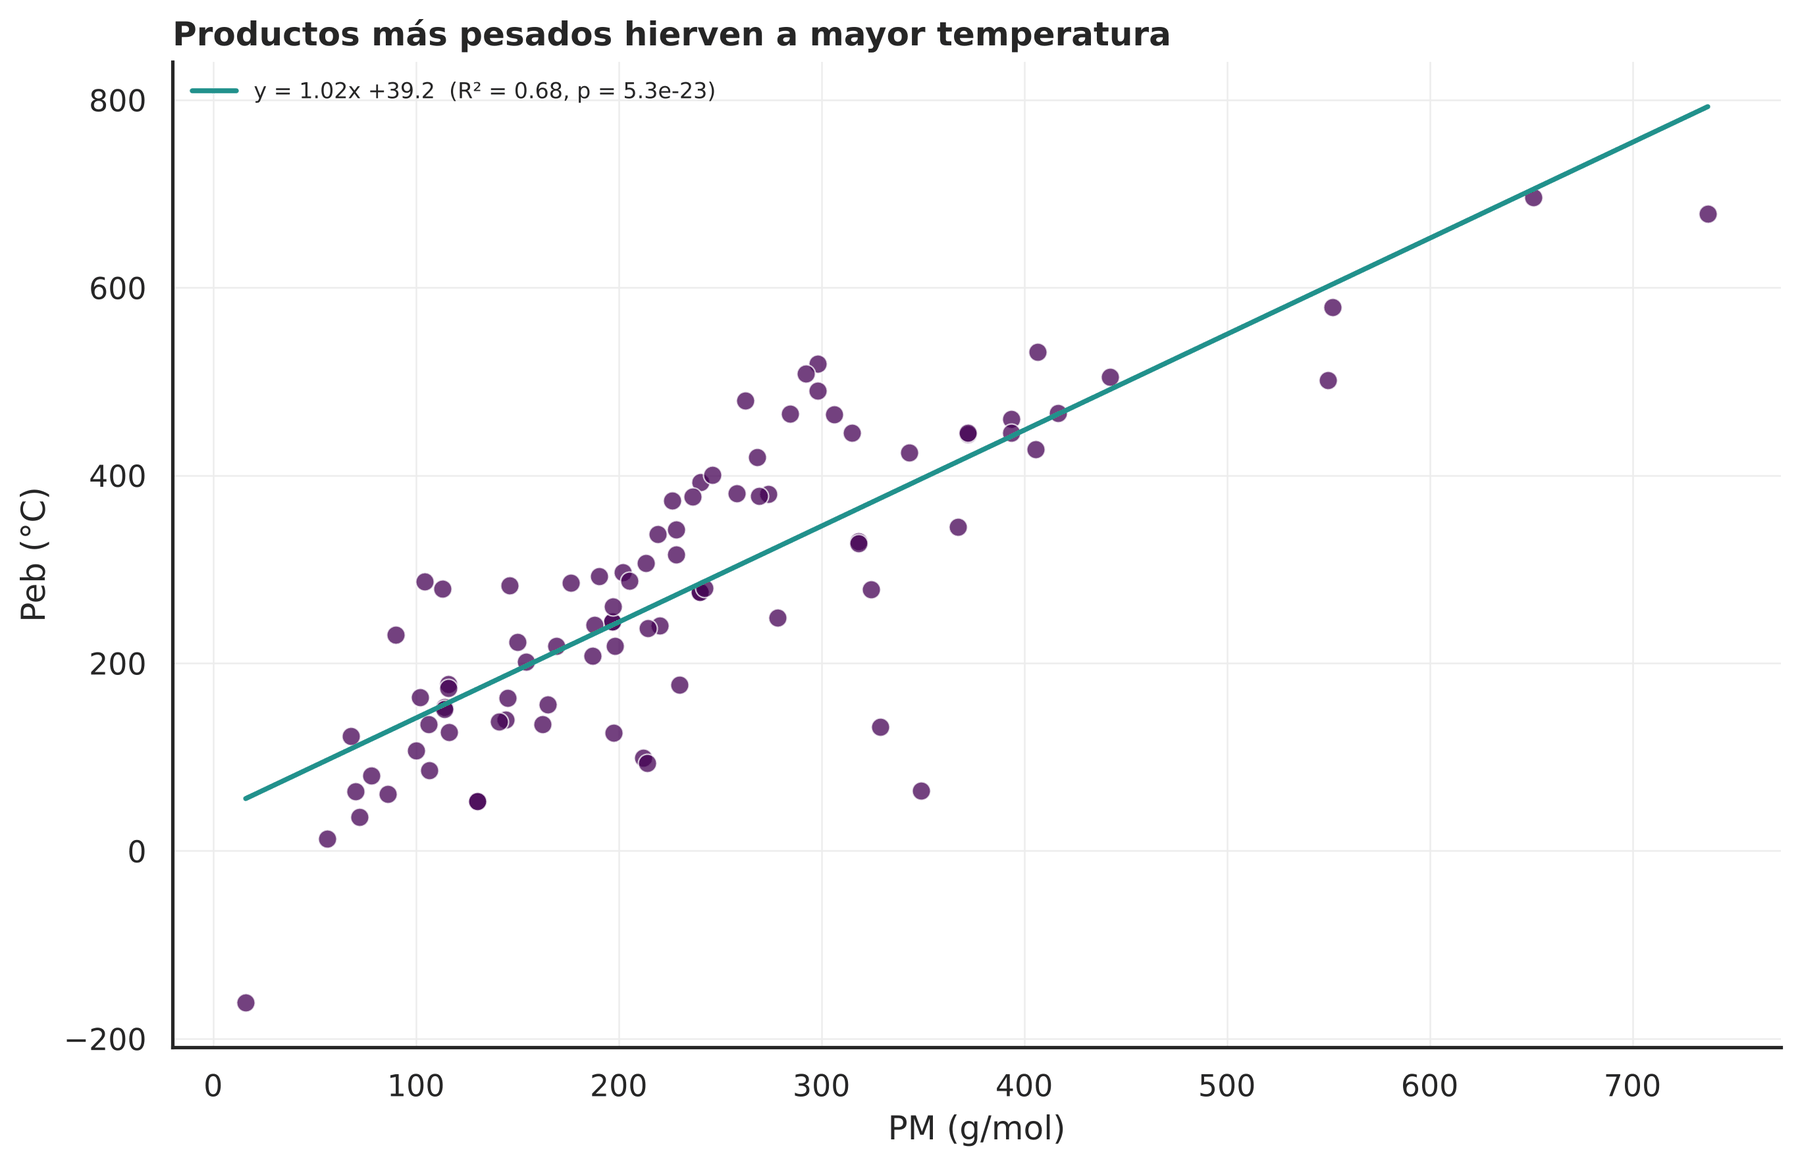
\includegraphics[width=\linewidth]{05_PM_vs_Peb.png}
\caption{PM frente a Peb.}
\label{fig:pmpeb}
\end{subfigure}\hfill
\begin{subfigure}[t]{0.329\textwidth}\centering
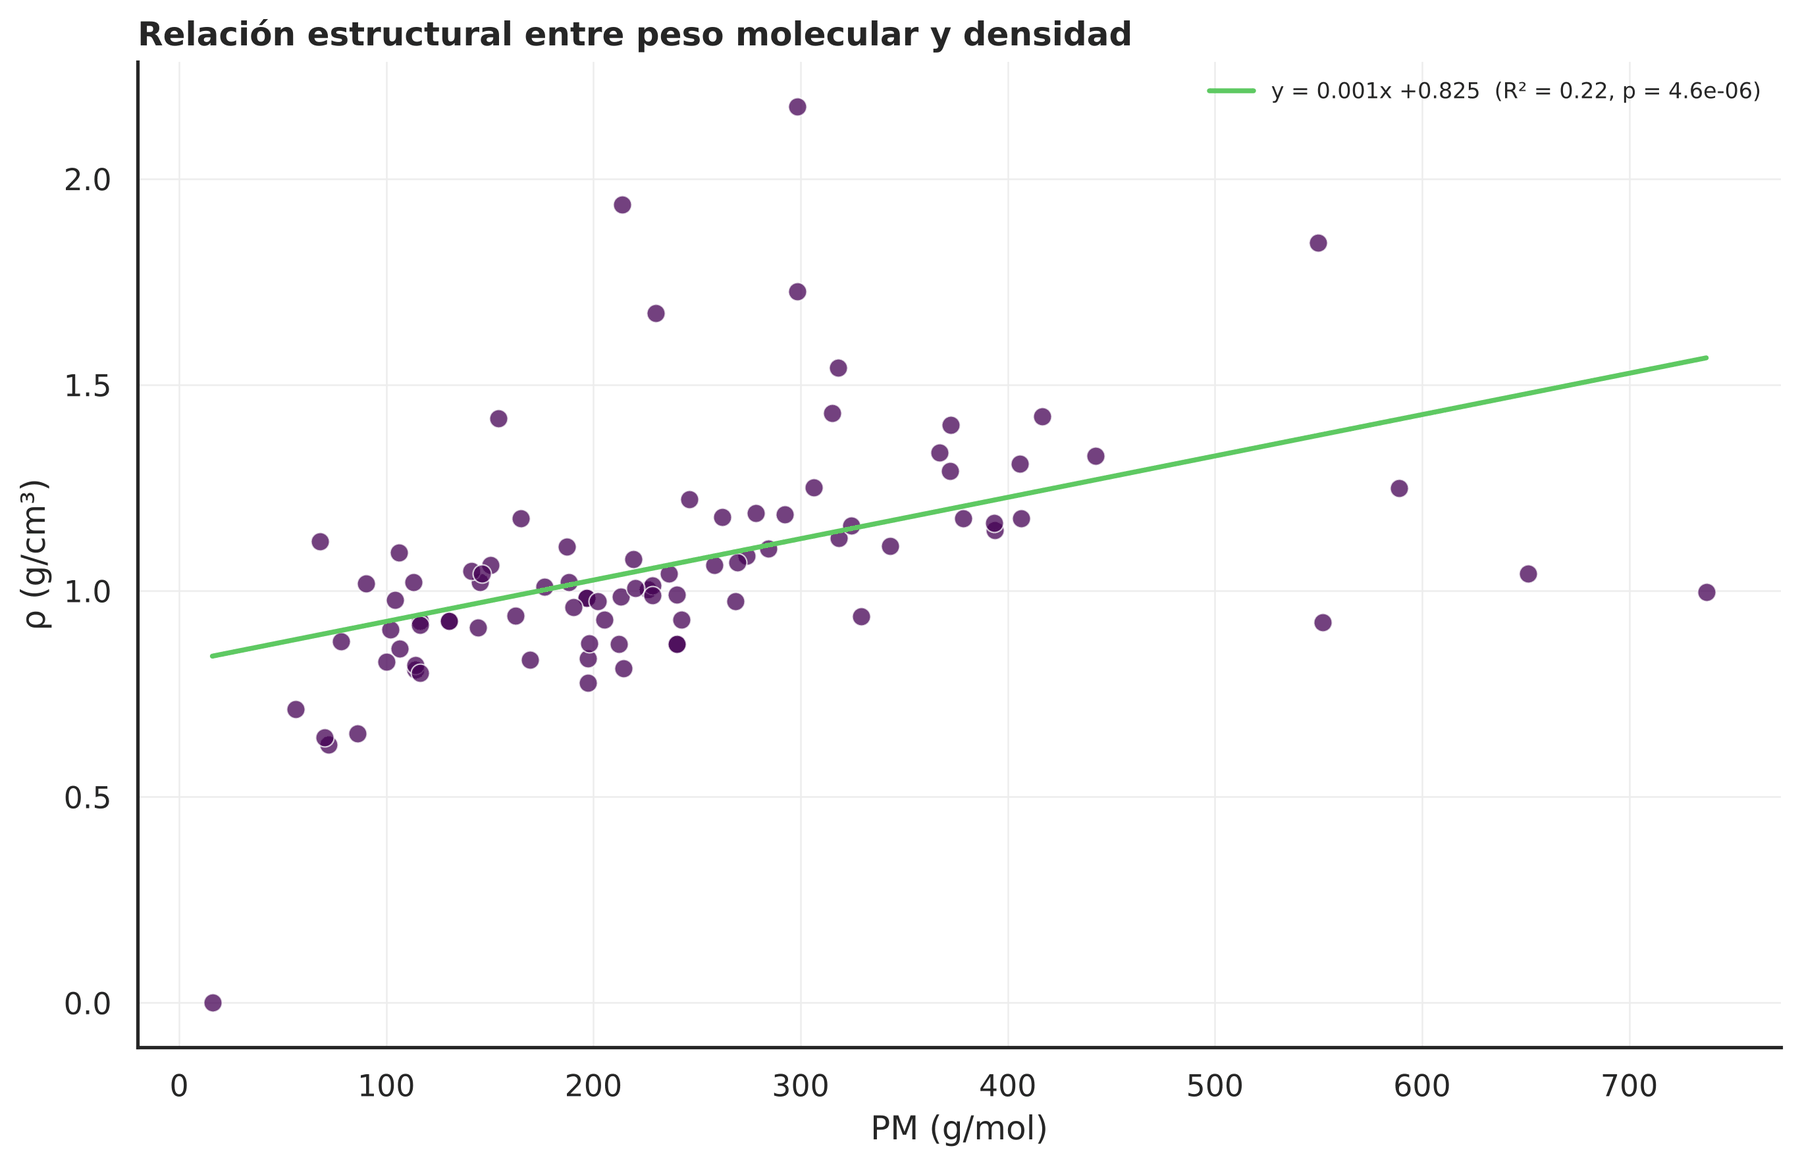
\includegraphics[width=\linewidth]{06_PM_vs_densidad.png}
\caption{PM frente a $\rho$.}
\label{fig:pmrho}
\end{subfigure}\hfill
\begin{subfigure}[t]{0.329\textwidth}\centering
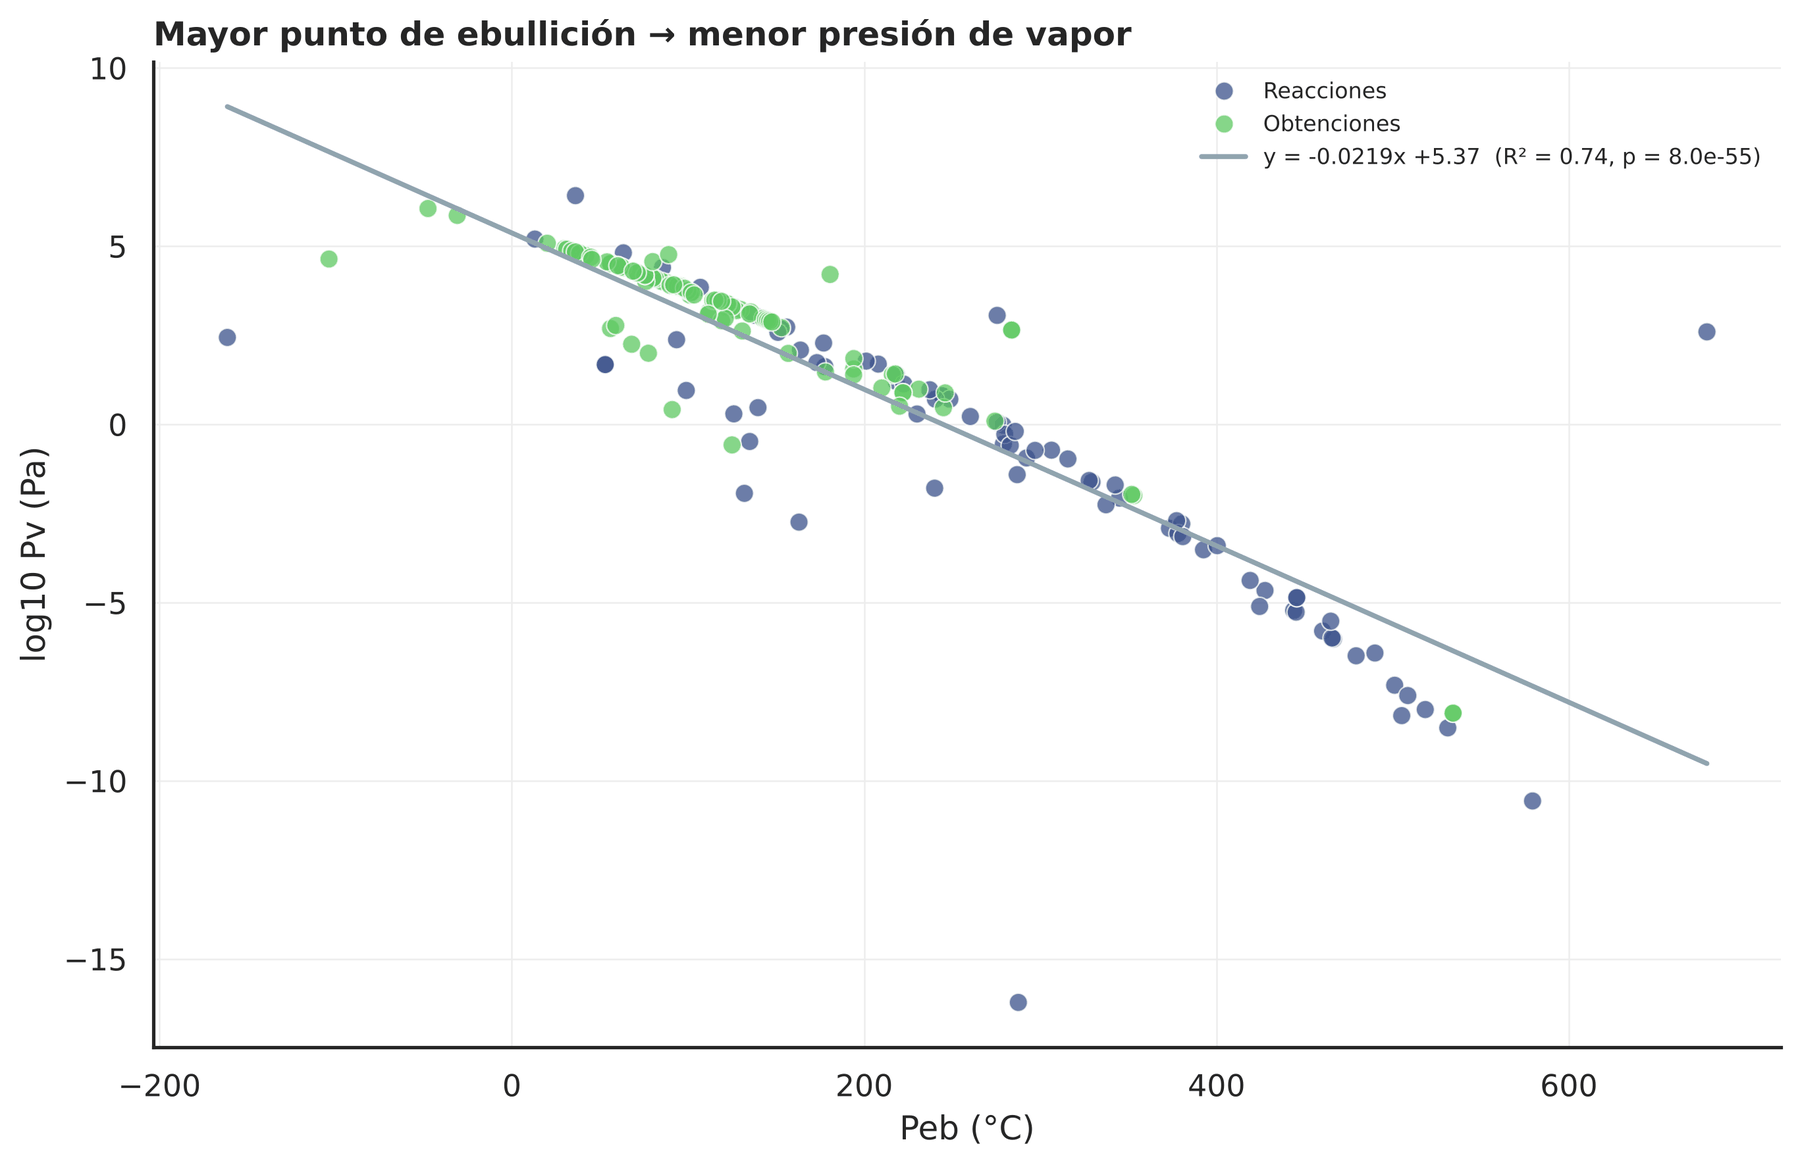
\includegraphics[width=\linewidth]{07_Peb_vs_Pv.png}
\caption{Peb frente a log Pv.}
\label{fig:pebpv}
\end{subfigure}
\caption{Relaciones entre propiedades de los productos de reacción (a, b) y de productos y reactivos (c), con su recta de regresión lineal.}
\label{fig:regresiones}
\end{figure*}

Los productos confirman la tendencia de las sustancias: Peb = 1.02·PM + 39 ($R^2$ = 0.68, $p$ = 5$\times$10$^{-23}$, $n$ = 88; Fig.~\ref{fig:pmpeb}) y log Pv = $-$0.022·Peb + 5.37 ($R^2$ = 0.74, $r$ = $-$0.86, $n$ = 184; Fig.~\ref{fig:pebpv}). Reactivos y productos se alinean sobre la misma recta, lo que indica que la relación entre punto de ebullición y presión de vapor es física y no depende del papel del compuesto en la reacción. La densidad aumenta con el PM solo de forma moderada ($R^2$ = 0.22; Spearman 0.63; Fig.~\ref{fig:pmrho}), porque depende de los heteroátomos que incorporan los productos.

\begin{figure*}[!t]
\centering
\begin{subfigure}[t]{0.49\textwidth}\centering
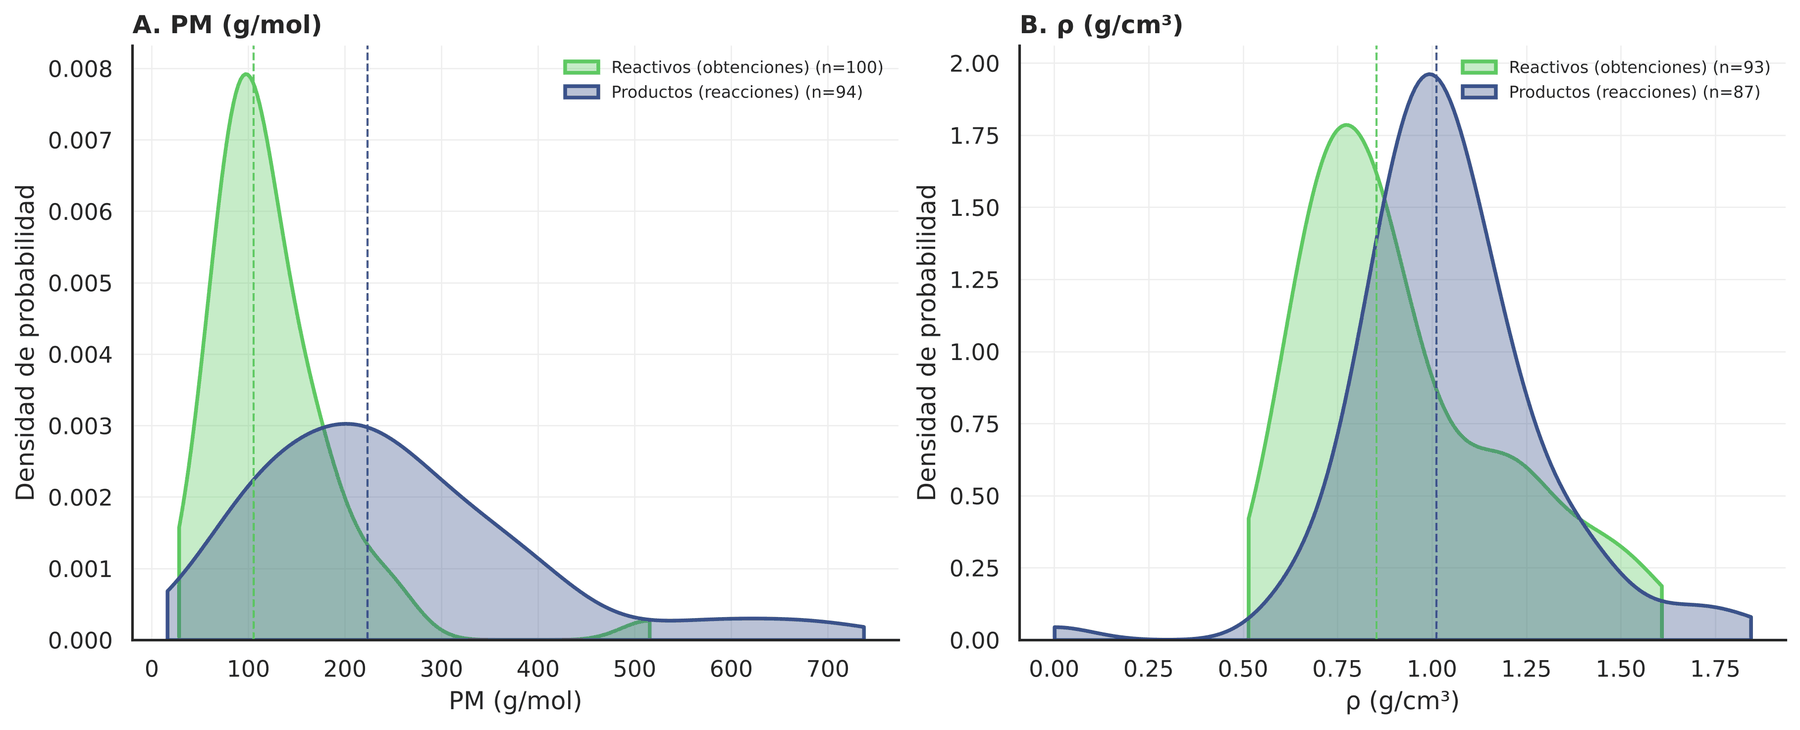
\includegraphics[width=\linewidth]{12_reactivos_vs_productos.png}
\caption{Densidad de probabilidad del PM (A) y de $\rho$ (B).}
\label{fig:kde}
\end{subfigure}\hfill
\begin{subfigure}[t]{0.49\textwidth}\centering
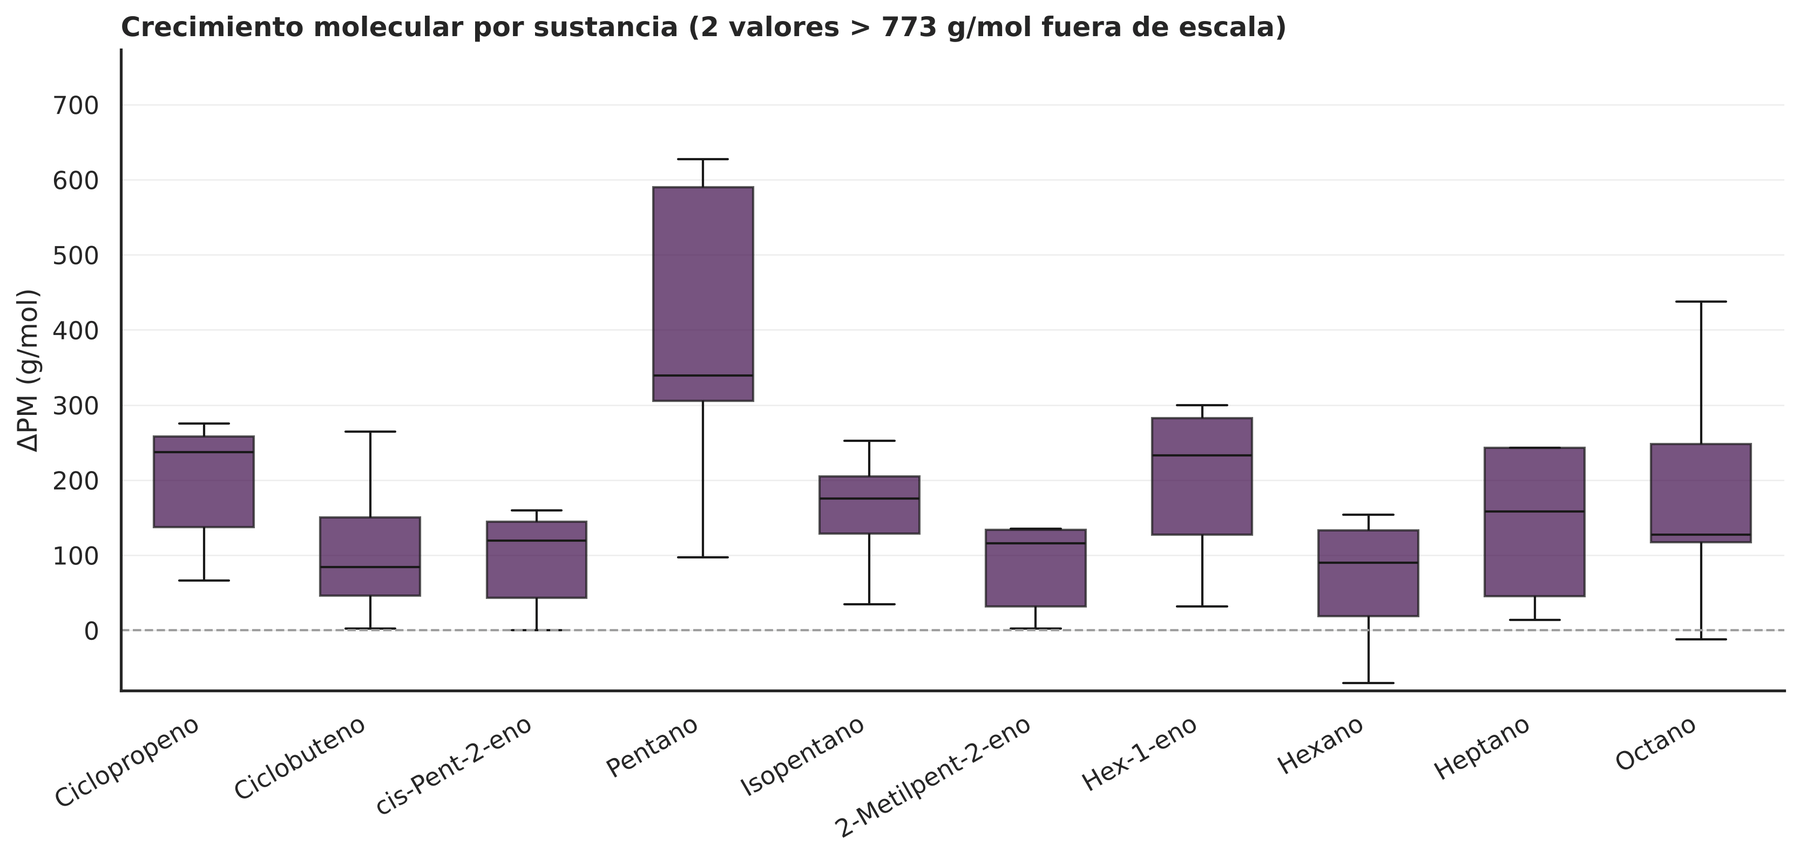
\includegraphics[width=\linewidth]{17_cambio_peso_molecular.png}
\caption{Cambio de peso molecular por hidrocarburo.}
\label{fig:dpm}
\end{subfigure}
\caption{Tamaño de reactivos y productos. Las líneas punteadas de (a) marcan las medianas; en (b), $\Delta$PM = PM del producto $-$ PM del hidrocarburo.}
\label{fig:tamano}
\end{figure*}

Los productos tienen una mediana de 228~g/mol, frente a 105~g/mol de los reactivos usados para obtener los hidrocarburos (Mann-Whitney $p$ = 1$\times$10$^{-14}$), y también son más densos (1.02 frente a 0.85~g/cm\textsuperscript{3}; $p$ = 4$\times$10$^{-5}$; Fig.~\ref{fig:kde}). En el 93\,\% de las reacciones el producto es más pesado que el hidrocarburo de partida (Fig.~\ref{fig:dpm}); el pentano presenta el mayor aumento (mediana +339~g/mol) porque en sus reacciones organometálicas se une a moléculas grandes.

\subsection{¿Cómo reaccionan y cómo se obtienen?}

\begin{figure*}[!t]
\centering
\begin{subfigure}[t]{0.47\textwidth}\centering
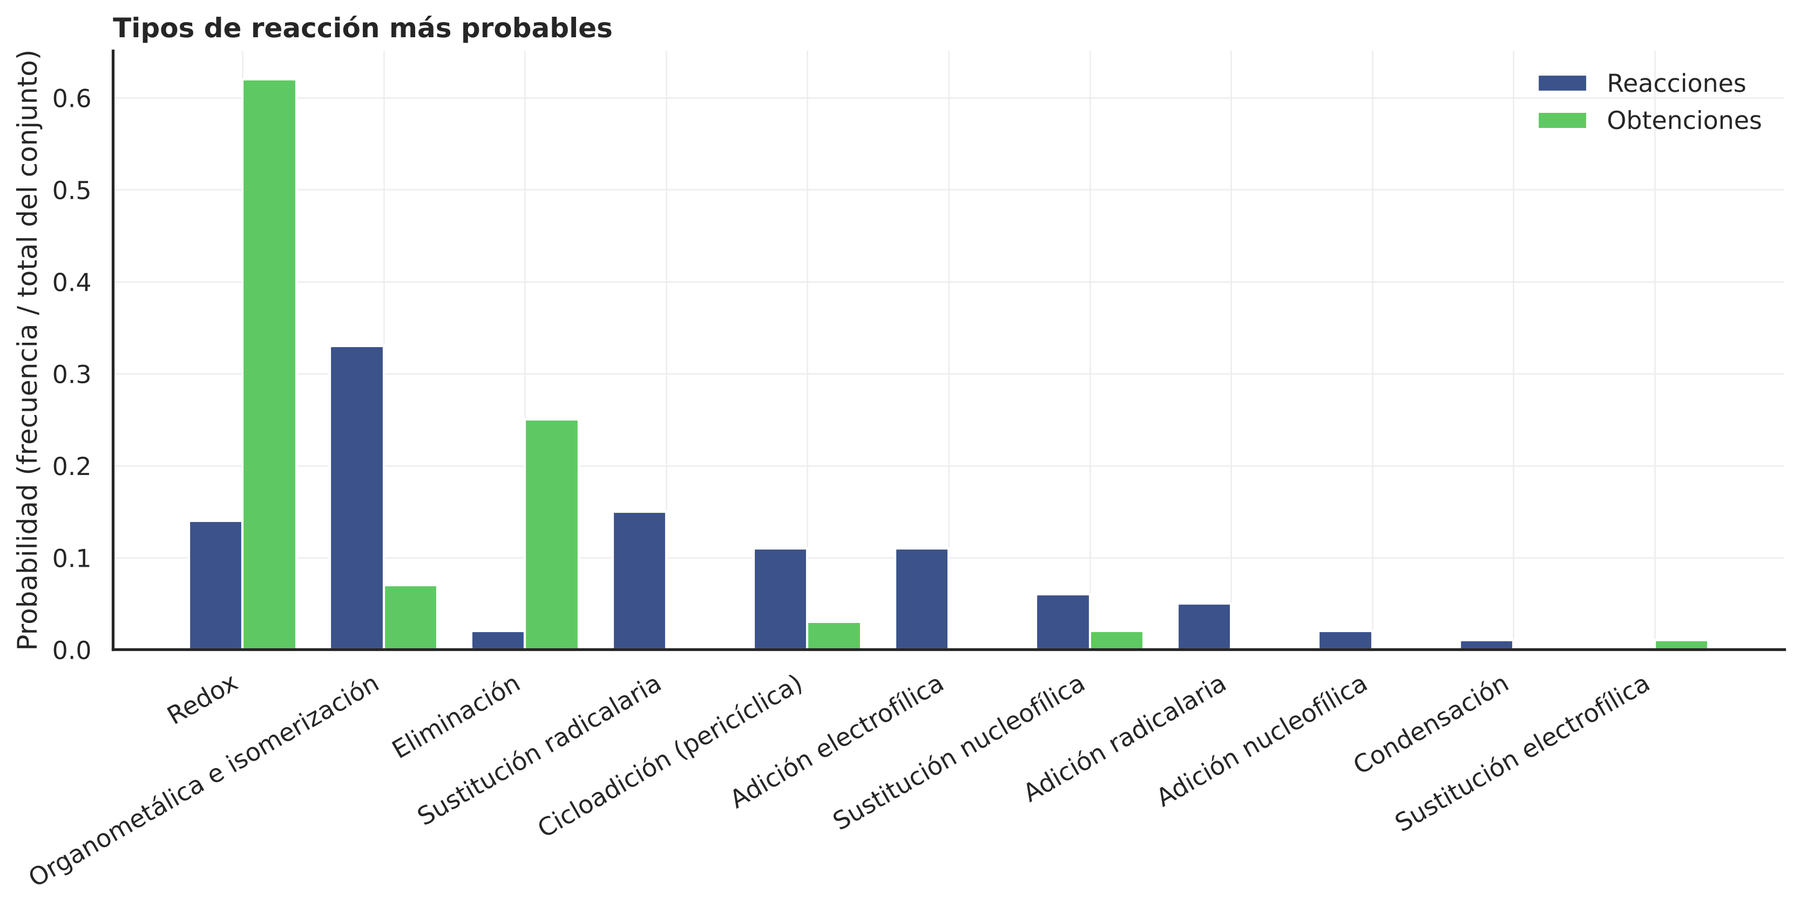
\includegraphics[width=\linewidth]{08_tipos_reaccion.png}
\caption{Probabilidad de cada tipo de reacción.}
\label{fig:tipos}
\end{subfigure}\hfill
\begin{subfigure}[t]{0.51\textwidth}\centering
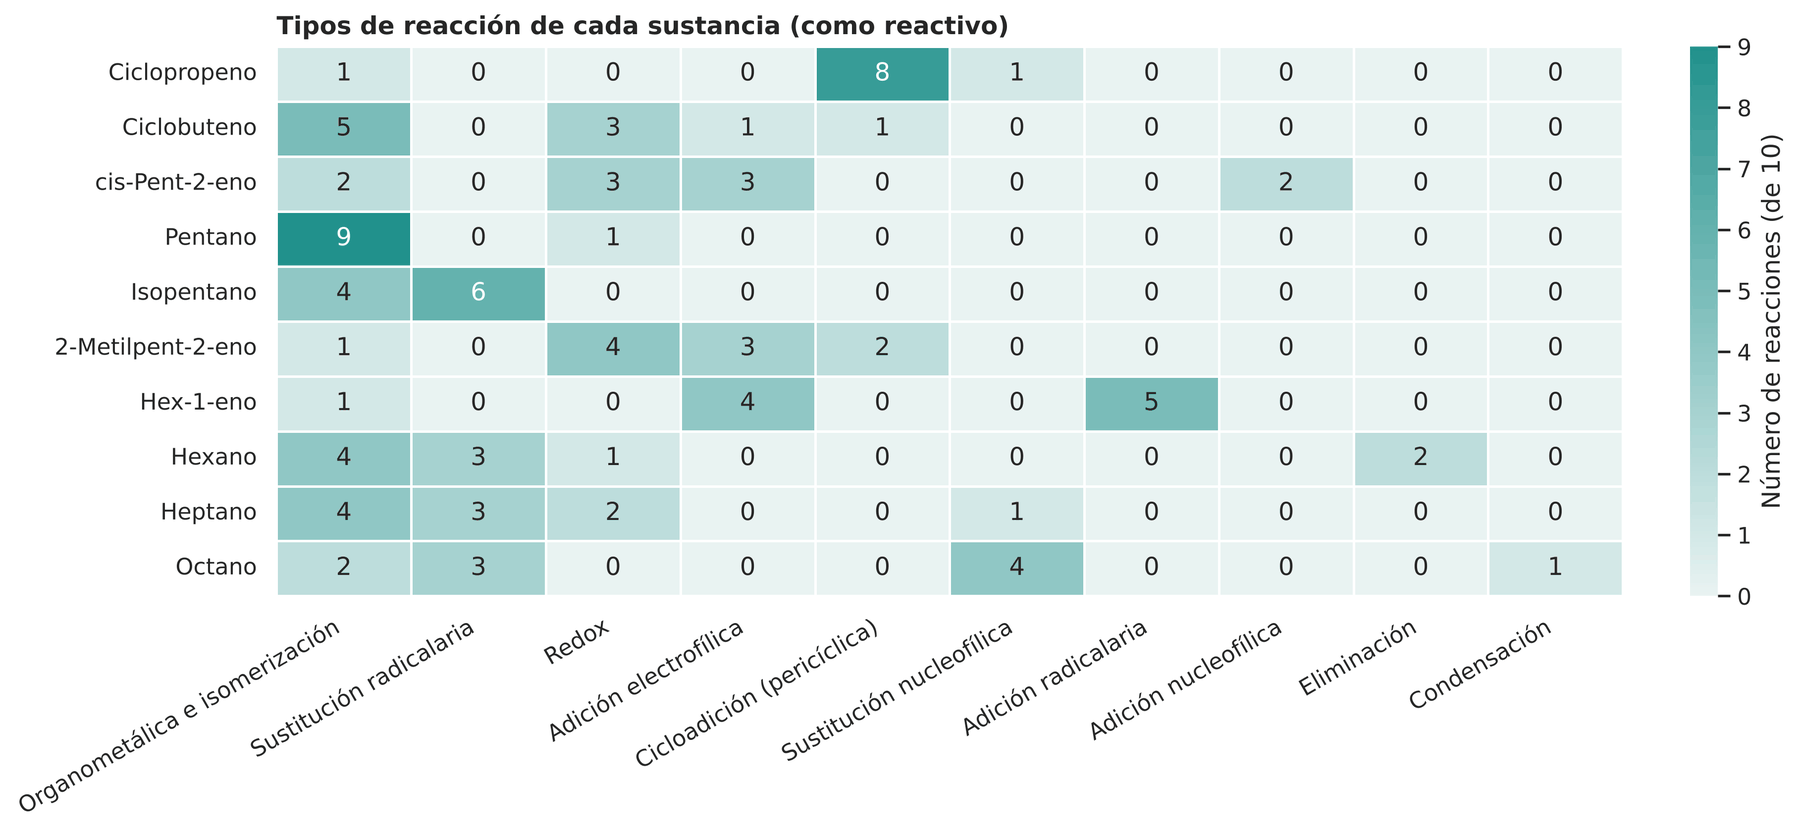
\includegraphics[width=\linewidth]{11_sustancia_tipo.png}
\caption{Tipo de reacción de cada hidrocarburo (como reactivo).}
\label{fig:sustipo}
\end{subfigure}
\caption{Mecanismos de reacción. En (a) se comparan las reacciones (el hidrocarburo es reactivo) con las obtenciones (el hidrocarburo es producto).}
\label{fig:mecanismos}
\end{figure*}

Cuando los hidrocarburos reaccionan, el tipo más frecuente es el organometálico (33\,\%; Fig.~\ref{fig:tipos}), seguido de la sustitución radicalaria (15\,\%): para romper un enlace C–H de alcano hace falta un metal de transición \cite{Labinger2002} o un radical generado, por ejemplo, por fotocatálisis \cite{HolmbergDouglas2022}. La Fig.~\ref{fig:sustipo} muestra la diferencia entre familias: el pentano reacciona por vía organometálica en 9 de 10 casos y el isopentano por vía radicalaria en 6, mientras que los alquenos reaccionan por adición (hex-1-eno: 5 radicalarias y 4 electrofílicas) y el ciclopropeno por cicloadición en 8 de 10, por la tensión de su anillo \cite{Kumar2018}. Para obtener los hidrocarburos domina el redox (62\,\%), sobre todo hidrogenaciones de alquenos y alquinos y reducciones de haluros \cite{Gong2025}, seguido de la eliminación (25\,\%), que forma los dobles enlaces de los alquenos.

\begin{figure*}[!t]
\centering
\begin{subfigure}[t]{0.42\textwidth}\centering
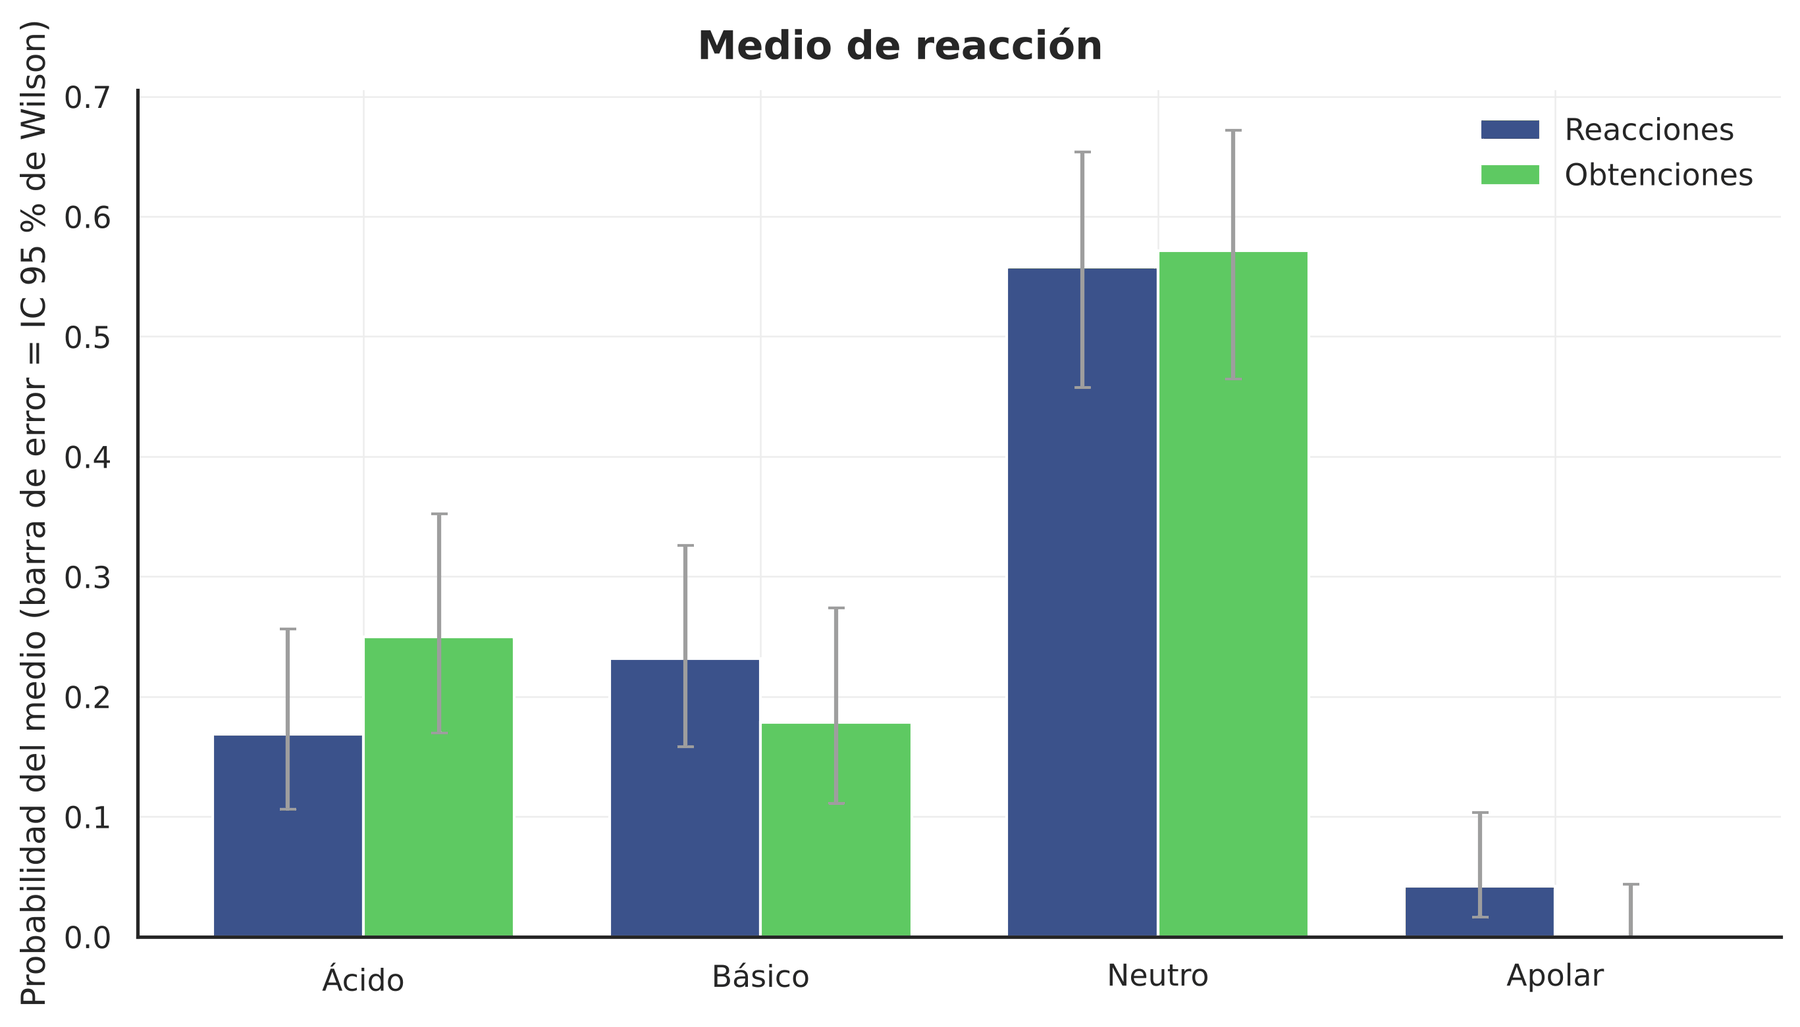
\includegraphics[width=\linewidth]{09_medio_reaccion.png}
\caption{Medio de reacción con IC 95\,\% de Wilson.}
\label{fig:medio}
\end{subfigure}\hfill
\begin{subfigure}[t]{0.56\textwidth}\centering
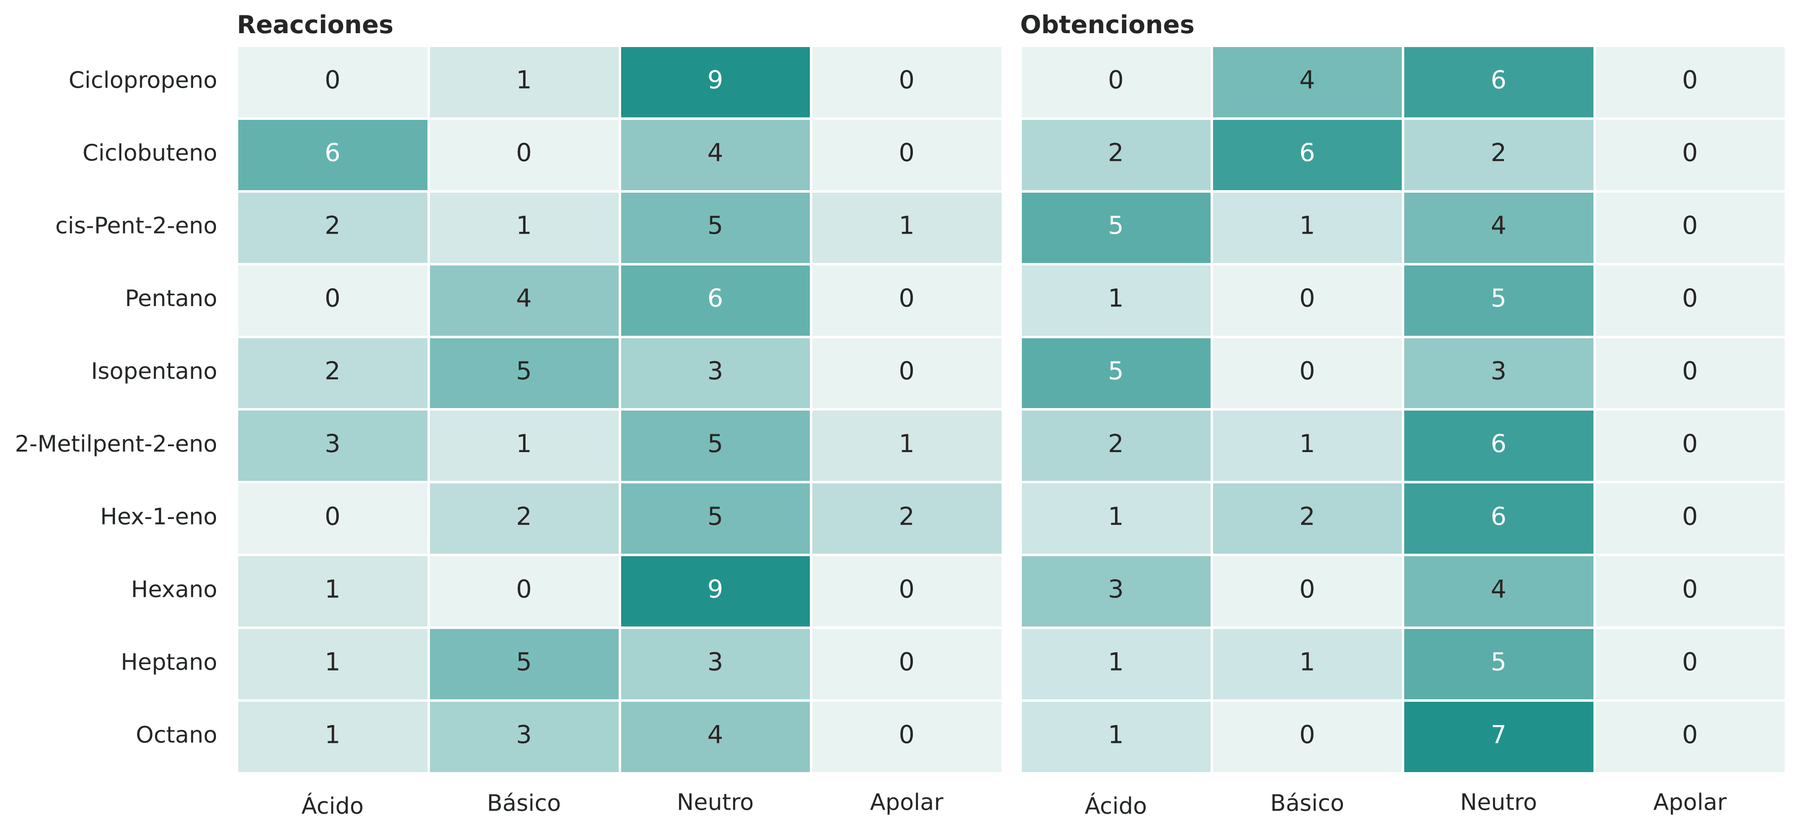
\includegraphics[width=\linewidth]{10_sustancia_medio.png}
\caption{Medio de cada hidrocarburo: reacciones (izquierda) y obtenciones (derecha).}
\label{fig:susmedio}
\end{subfigure}
\caption{Medio de reacción.}
\label{fig:medios}
\end{figure*}

El medio neutro es claramente el más probable, con 0.56 [0.46–0.65] en reacciones y 0.57 [0.46–0.67] en obtenciones (Fig.~\ref{fig:medio}), y su intervalo no se solapa con los de los demás medios. Esto es coherente con sustancias sin grupos ácidos ni básicos. El ciclopropeno y el hexano reaccionan en medio neutro en 9 de 10 casos, y el ciclobuteno se obtiene sobre todo en medio básico (6 de 10), en eliminaciones con bases fuertes (Fig.~\ref{fig:susmedio}).

\subsection{Condiciones de reacción}

Las obtenciones requieren calentamiento con mayor probabilidad que las reacciones (0.68 [0.56–0.77] frente a 0.57 [0.45–0.67]; medianas de 60 y 40~\textdegree C; Fig.~\ref{fig:temp}). Los valores extremos corresponden a la deshidrogenación y la deshidroaromatización del hexano (400 y 525~\textdegree C) y a reacciones enfriadas hasta $-$75~\textdegree C. La probabilidad de calentar es parecida en los tres medios (0.61–0.69), pero cuando se calienta en medio ácido las obtenciones alcanzan una mediana de 150~\textdegree C, propia de las deshidrataciones de alcoholes (Fig.~\ref{fig:tempmedio}).

\begin{figure*}[!t]
\centering
\begin{subfigure}[t]{0.47\textwidth}\centering
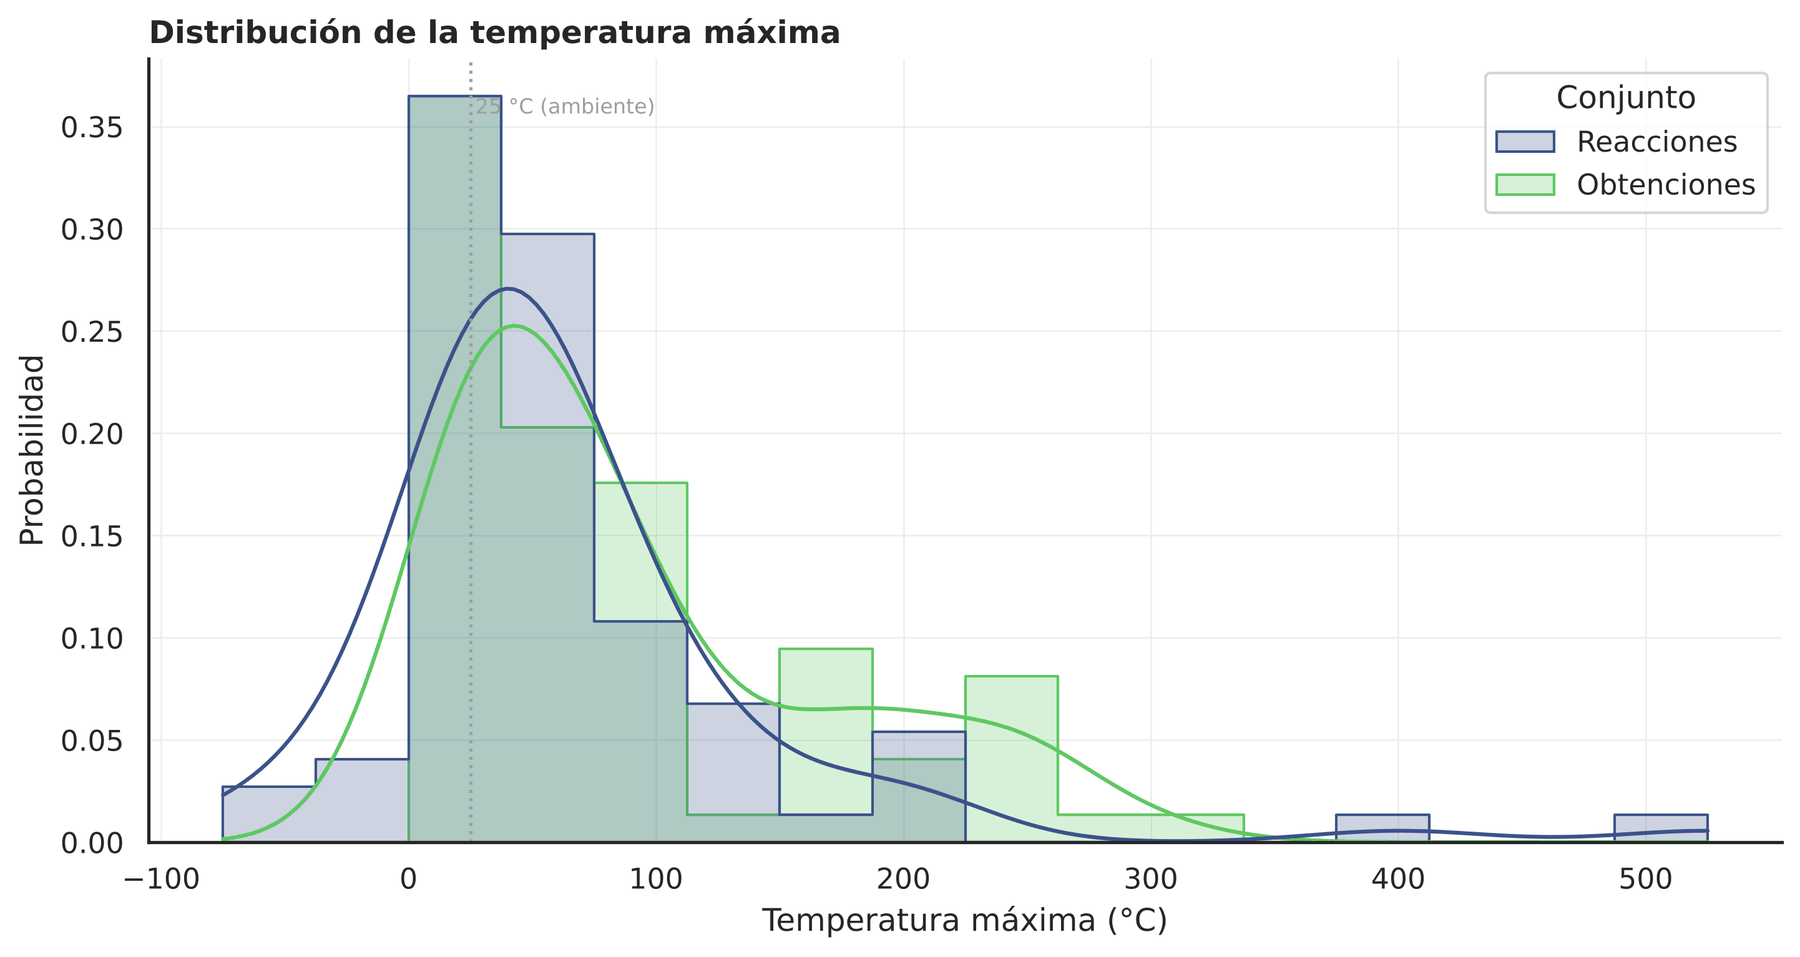
\includegraphics[width=\linewidth]{13_distribucion_temperatura.png}
\caption{Distribución de la temperatura máxima.}
\label{fig:temp}
\end{subfigure}\hfill
\begin{subfigure}[t]{0.51\textwidth}\centering
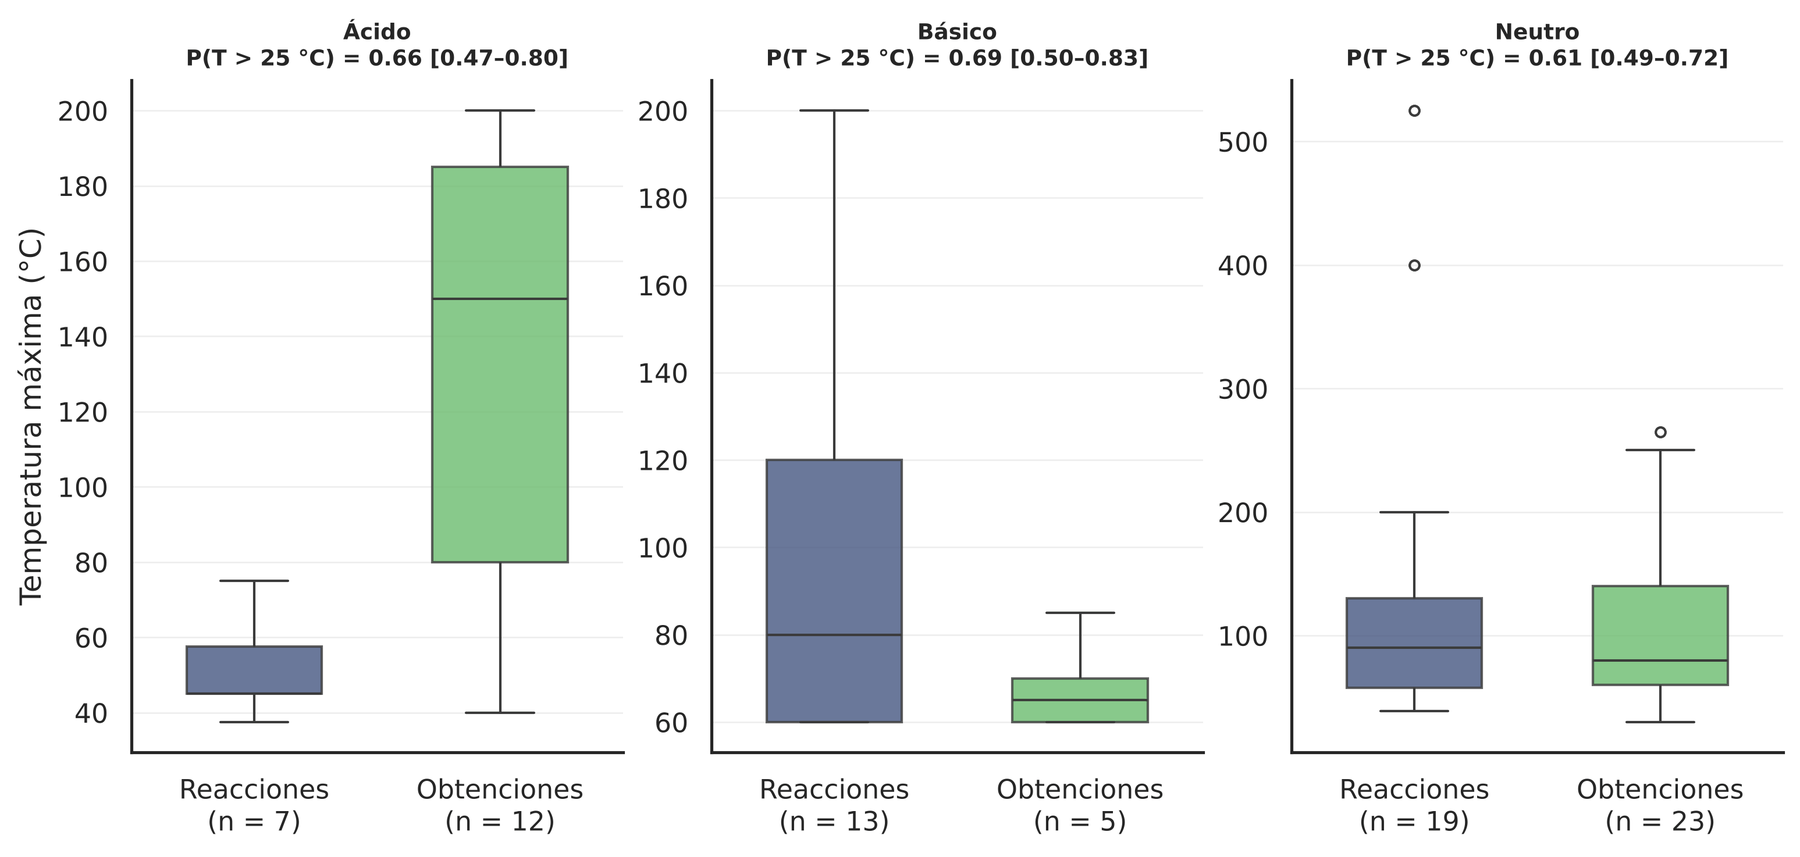
\includegraphics[width=\linewidth]{14_temperatura_por_medio.png}
\caption{Temperatura de las reacciones con calentamiento, por medio.}
\label{fig:tempmedio}
\end{subfigure}
\caption{Temperatura de reacción. En (b) solo se incluyen reacciones con T $>$ 25~\textdegree C y cajas con al menos cinco datos.}
\label{fig:temperatura}
\end{figure*}



\begin{figure*}[!t]
\centering
\begin{subfigure}[t]{0.49\textwidth}\centering
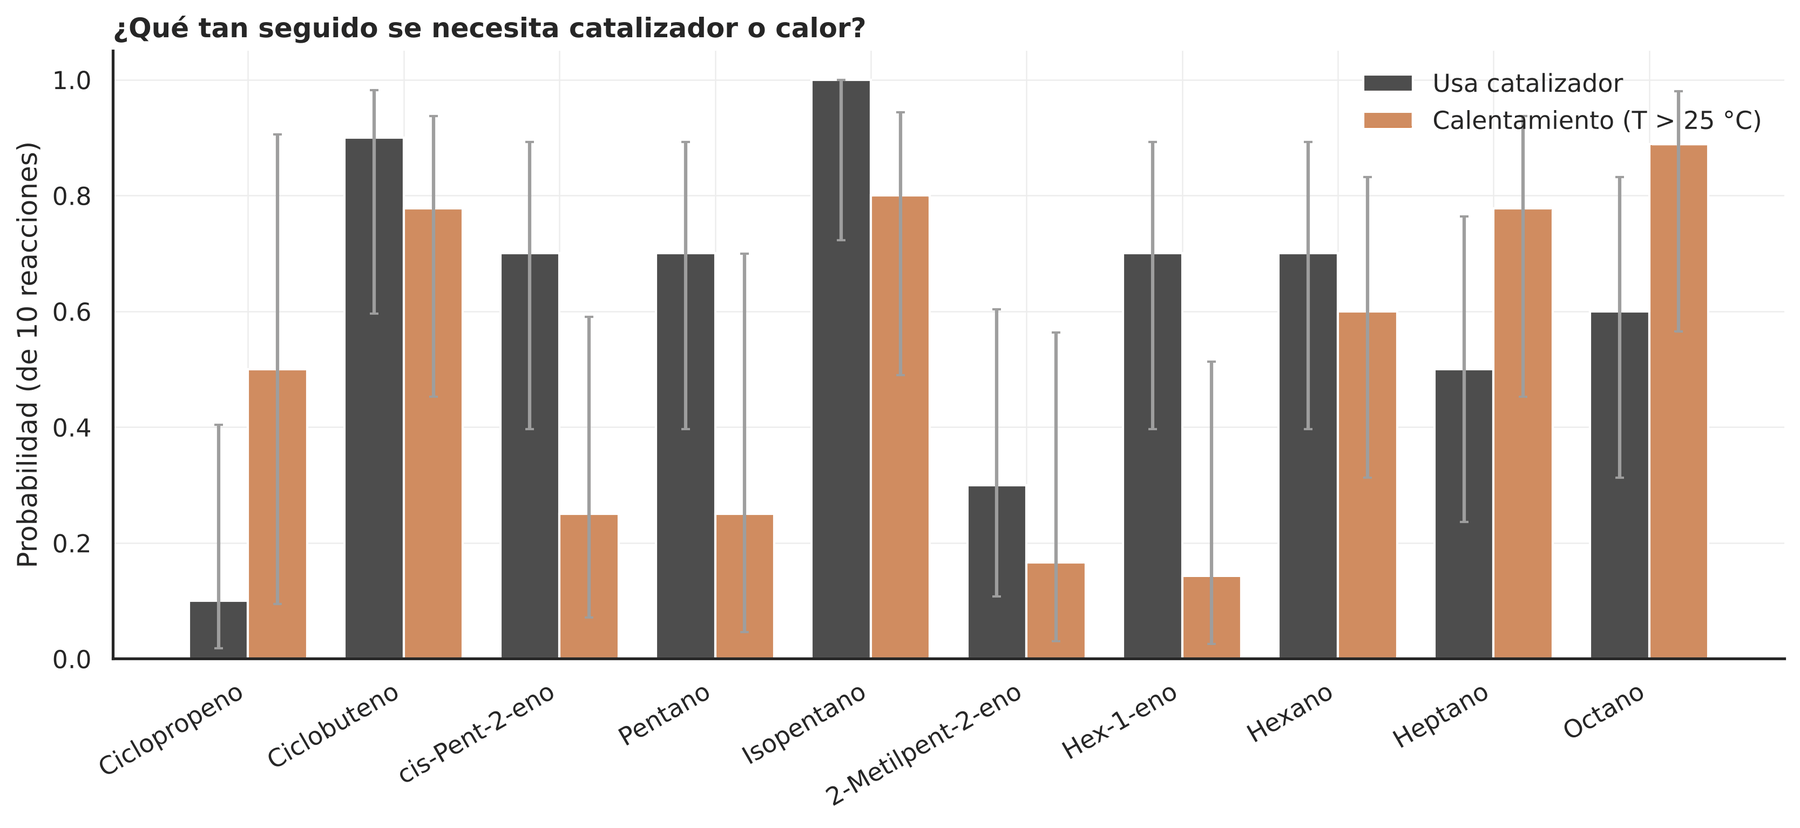
\includegraphics[width=\linewidth]{15_prob_catalizador_calor.png}
\caption{Probabilidad de usar catalizador y de calentar.}
\label{fig:catcalor}
\end{subfigure}\hfill
\begin{subfigure}[t]{0.49\textwidth}\centering
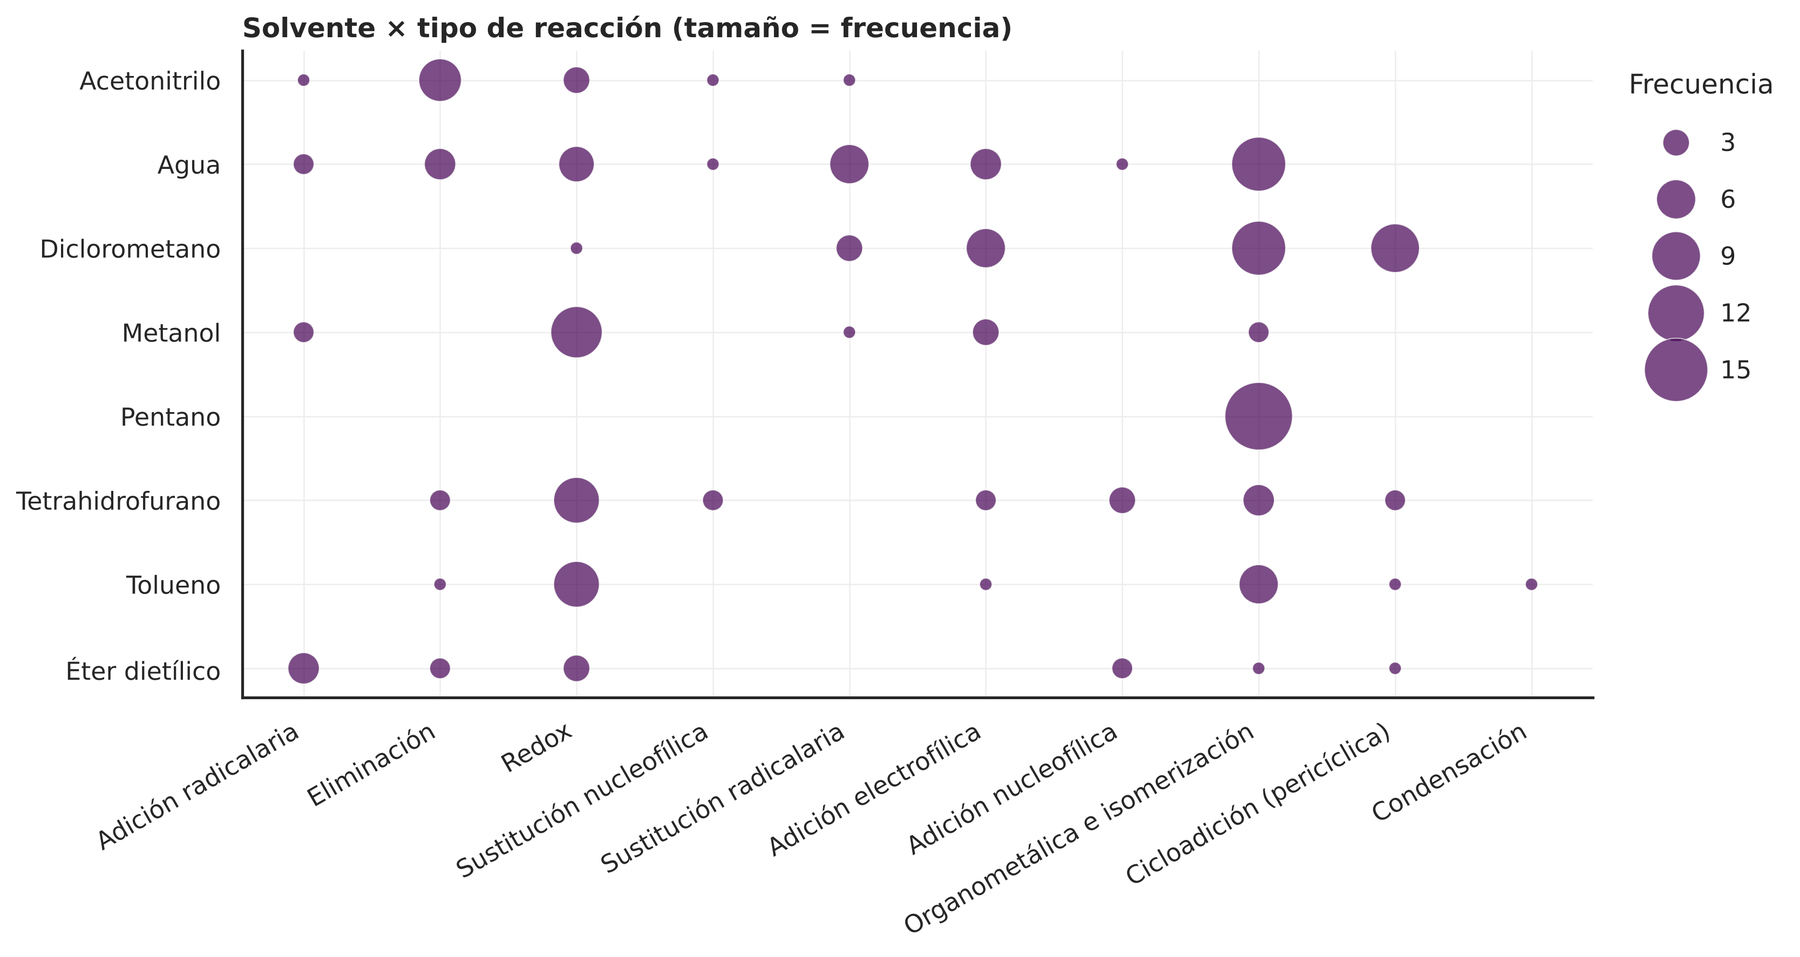
\includegraphics[width=\linewidth]{16_burbujas_solvente_tipo.png}
\caption{Solvente frente a tipo de reacción.}
\label{fig:burbujas}
\end{subfigure}
\caption{Catalizador, calentamiento y solventes de las reacciones de cada hidrocarburo. Las barras de error de (a) son el IC 95\,\% de Wilson.}
\label{fig:condiciones}
\end{figure*}

El 62\,\% de las reacciones usa catalizador, y esa proporción sube a 0.83 cuando hay calentamiento ($n$ = 42), frente a 0.56 sin calentamiento ($n$ = 32; Fig.~\ref{fig:catcalor}). El isopentano usa catalizador en todas sus reacciones y el ciclopropeno solo en una, porque su anillo tensionado reacciona sin ayuda. Entre los solventes (Fig.~\ref{fig:burbujas}), el pentano en reacciones organometálicas es la combinación más frecuente (17), seguido del diclorometano y el agua en el mismo tipo de reacción (11 cada uno) y del metanol en hidrogenaciones (10). La Fig.~\ref{fig:interactivas} muestra capturas de las gráficas interactivas que se encuentran en el colab que puede verse en el repositorio del grupo en donde se puede interactuar con estas.

\begin{figure*}[!t]
\centering
\begin{subfigure}[t]{0.49\textwidth}\centering
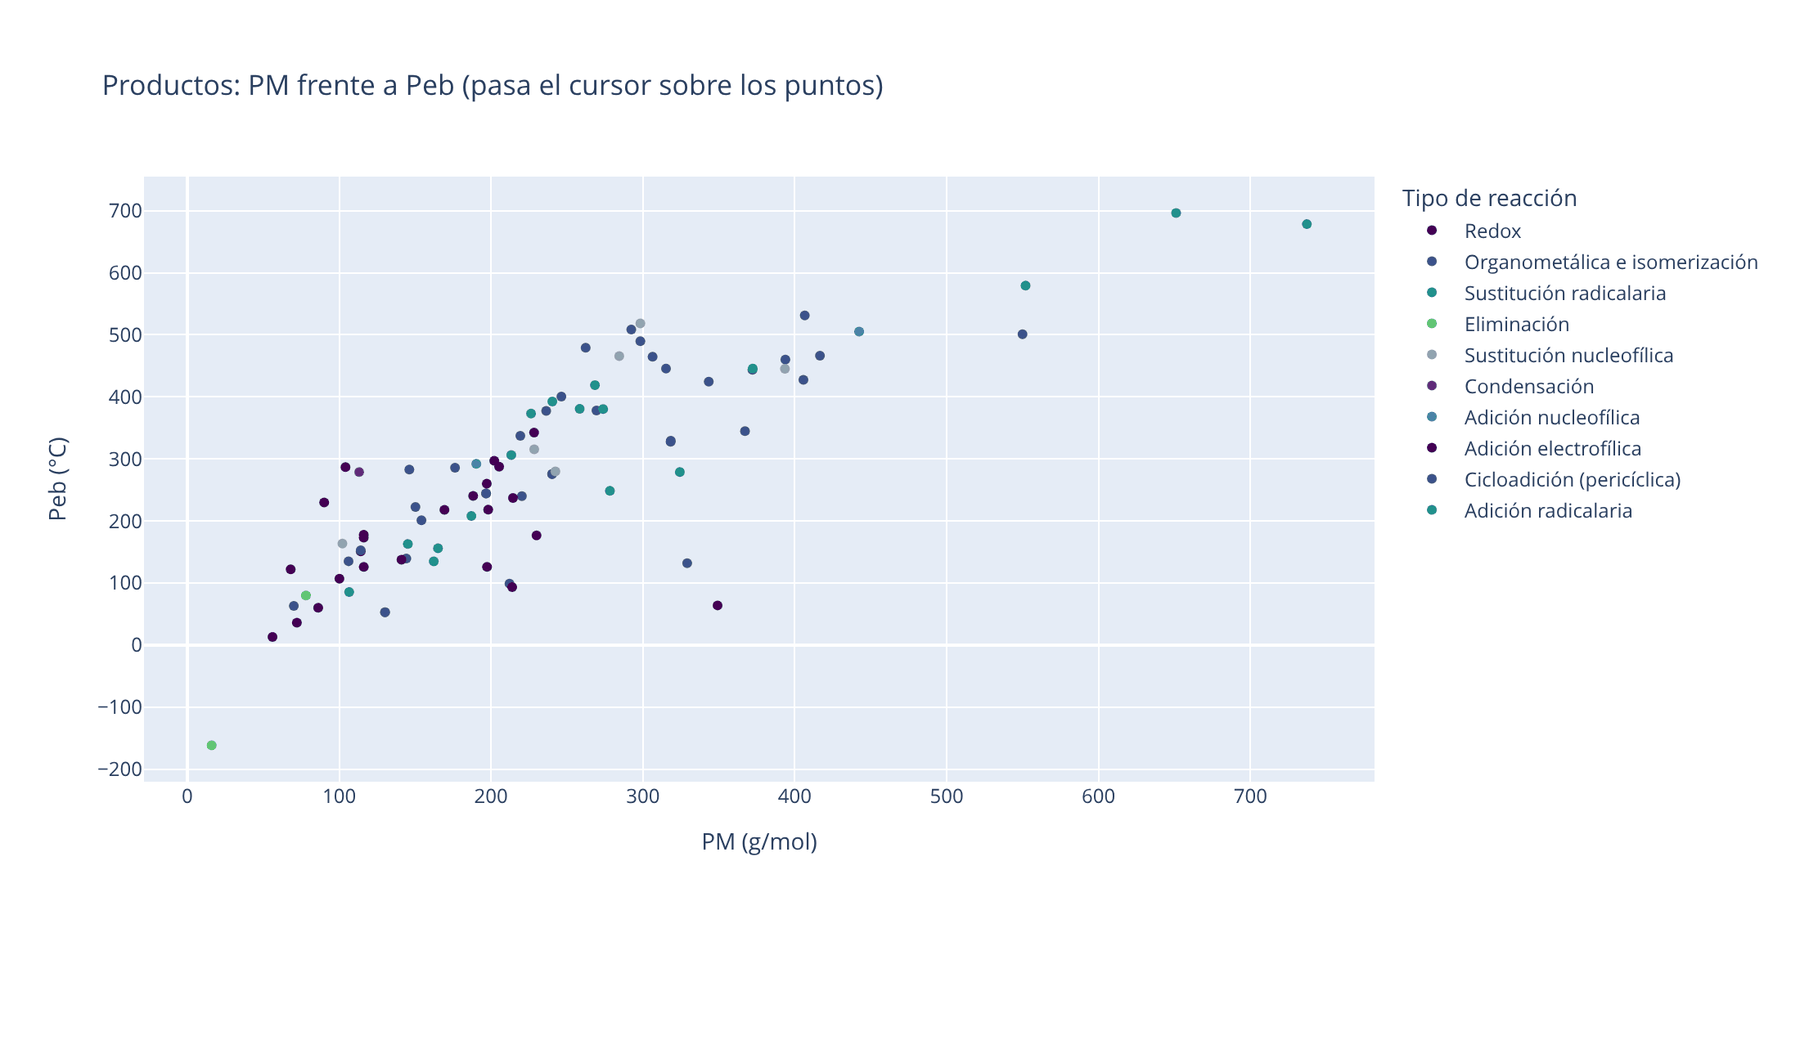
\includegraphics[width=\linewidth]{18_interactivo_PM_Peb.png}
\caption{Dispersión PM–Peb por tipo de reacción.}
\end{subfigure}\hfill
\begin{subfigure}[t]{0.49\textwidth}\centering
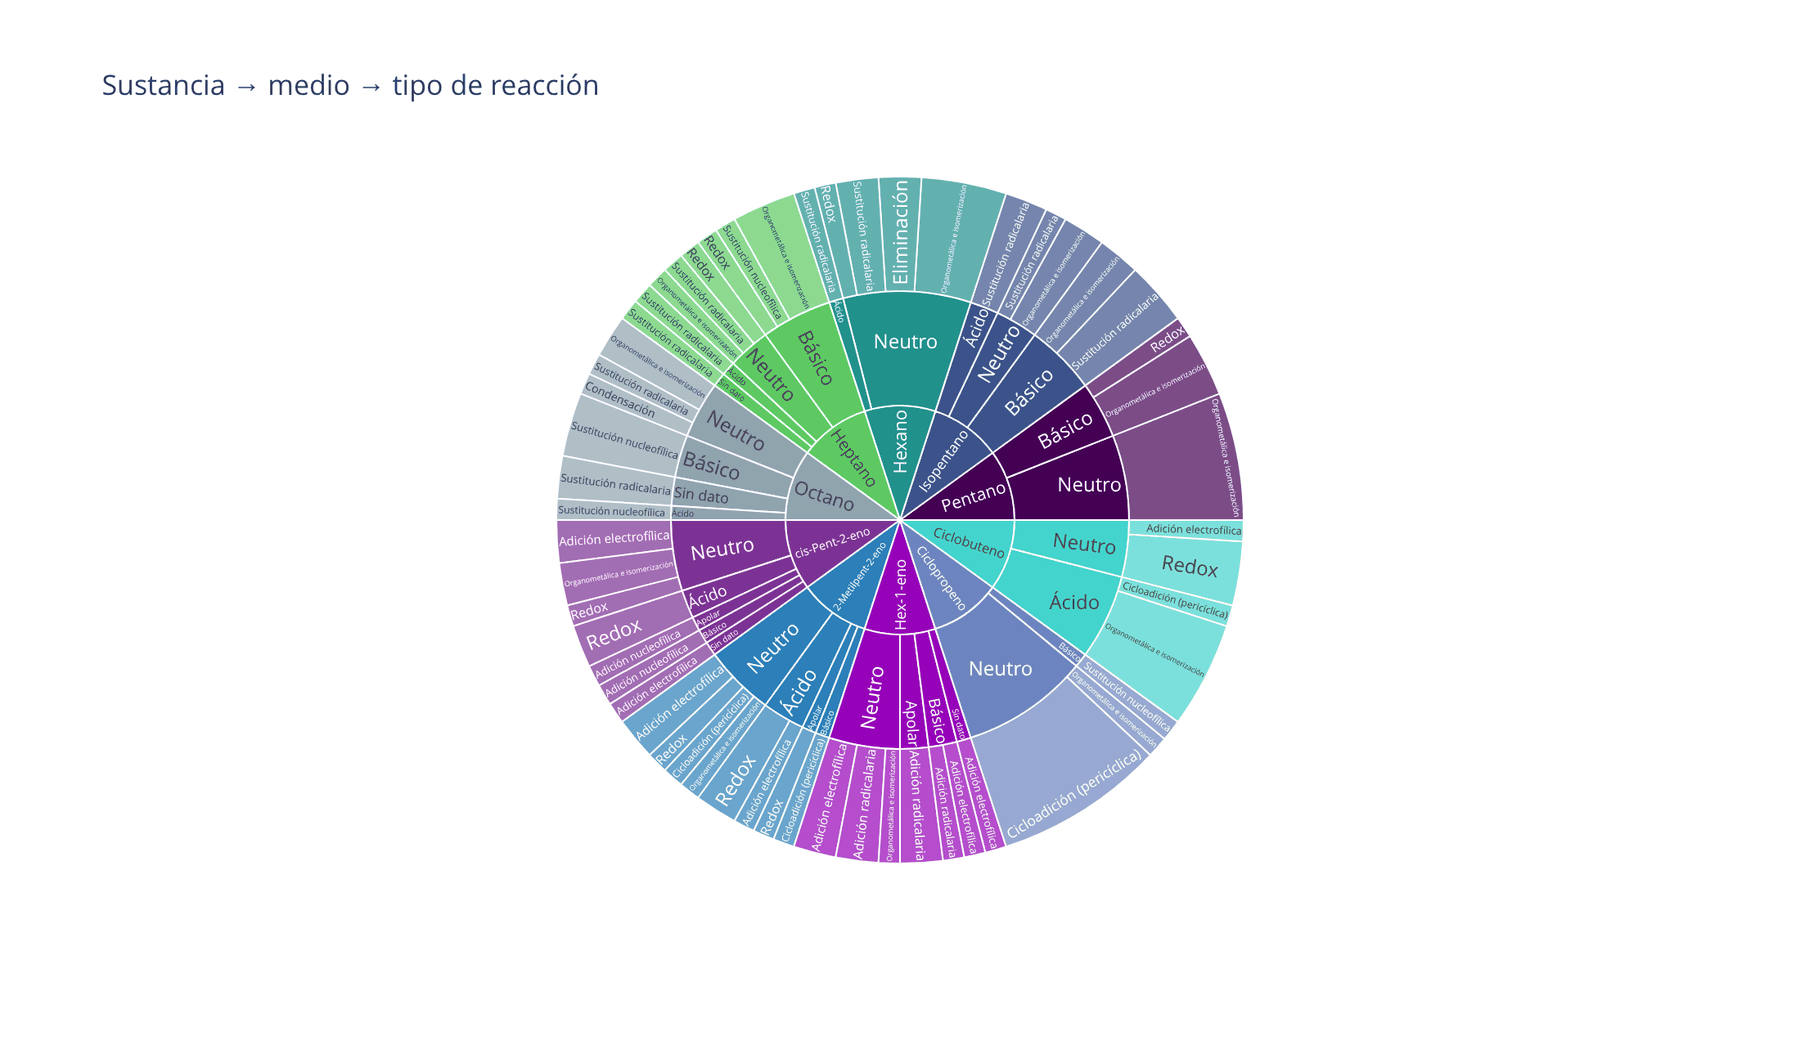
\includegraphics[width=\linewidth]{19_interactivo_solar.png}
\caption{Diagrama solar sustancia $\rightarrow$ medio $\rightarrow$ tipo.}
\end{subfigure}
\caption{Capturas de las gráficas interactivas elaboradas con Plotly.}
\label{fig:interactivas}
\end{figure*}

\subsection{Limitaciones}
Cada hidrocarburo tiene diez reacciones y diez obtenciones, de modo que los resultados describen este conjunto de datos y no toda su química, se observo que si bien algunos elementos tenian una amplia gama de información en la que es posible hacer un filtro de las reacciones o obtenciones que esten mas completas, tambien se vieron casos en donde las reaccione y obtenciones era muy poca en algunos casos fue casi que exacta para las 10 que se necesitaban lo que dificulta el filtro y nos puede dar errores en esta información al no tener con que compararla.

\section{Conclusiones y Perspectiva}
\fontsize{12}{14}\selectfont
Las propiedades físicas de los hidrocarburos dependen del tamaño y la forma de la molécula: cada carbono adicional en la serie lineal sube el punto de ebullición unos 30~\textdegree C, la ramificación lo reduce y, en los productos, la presión de vapor disminuye de forma marcada al aumentar el punto de ebullición, en cuanto a la reactividad, el tipo de hidrocarburo determina el mecanismo: los alcanos necesitan metales o radicales para romper el enlace C–H, los alquenos reaccionan por adición y el ciclopropeno por cicloadición, para obtenerlos predominan la reducción y la eliminación y la mayoría de las reacciones ocurre en medio neutro y con catalizador.


\textbf{Contribución de los autores:}

Integrante 1 y  2: búsqueda en SciFinder y tabla de datos. Integrante 2: análisis en Google Colab. Integrante 3: informe en LaTeX. Integrante 4: tablero en Power BI. Todos revisaron y aprobaron el documento.

\textbf{Disponibilidad de datos y código:} La tabla de datos, el cuaderno de Google Colab y el tablero de Power BI se encuentran en el repositorio de GitHub del grupo.

\printbibliography

\end{document}